\documentclass[12pt,a4paper]{article}

\input{glyphtounicode}
\pdfgentounicode=1
\usepackage[utf8]{inputenc}
\usepackage{cmap}
\usepackage[T1]{fontenc}
\usepackage{xcolor}
\usepackage{hyperref}
\hypersetup{
	colorlinks=true,
	linkcolor=blue,
	filecolor=blue, 
	citecolor=blue,
	urlcolor=blue, 
	pdftitle={},
	pdfpagemode=FullScreen,
}
\usepackage{url}
\urlstyle{same}
\usepackage{booktabs}
\usepackage{amsfonts}
\usepackage{amsthm}
\usepackage{amsmath}
\usepackage{float}
\usepackage{graphicx}
\usepackage{caption}
\usepackage{nicefrac}
\usepackage[sort,numbers]{natbib}
\bibliographystyle{plainnat}
\usepackage[title]{appendix}
\usepackage{longtable}
\usepackage{listings}
\setcounter{secnumdepth}{3}
\let\oldcite\cite
\renewcommand{\cite}[1]{\mbox{\oldcite{#1}}}

\newtheorem{theorem}{Theorem}
\newtheorem{lemma}{Lemma}
\newtheorem{proposition}{Proposition}
\newtheorem{corollary}{Corollary}
\theoremstyle{definition}
\newtheorem{definition}{Definition}
\newtheorem{remark}{Remark}

\newlength{\extraspace}
\setlength{\extraspace}{\lineskip}

\voffset -1in
\topmargin 25mm
\headheight 4.3mm
\headsep 4mm
\textheight 238.7mm
\addtolength{\headsep}{2.5mm}

\hoffset -1in
\marginparwidth 0mm
\marginparsep 0mm
\evensidemargin 25mm
\oddsidemargin 25mm
\textwidth 160mm

\parindent 0mm
\parskip 2mm plus 1pt

\title{Planning as Autoregressive Sequence Modelling: Decoding Strategies}
\author{Dian Kruger \\ Shane Josias}
\date{}
\begin{document}

\maketitle

\section{Introduction}

Planning is a central problem in artificial intelligence, concerned with finding a sequence of
actions that moves an environment from an initial state to a desired goal state
~\cite{Alarnaouti2023planning}. In this project, the planning problem is studied in a discrete 2D
maze environment, where the task is to generate a valid trajectory from a given start position to a
specified goal position without passing through walls.

One way to approach such a problem is to treat trajectories as data and learn a probability
distribution over successful trajectories from examples. From this perspective, planning can be
viewed as inference in a learned generative model~\cite{janner2021trajectory}. If the model is trained on valid and efficient
demonstration trajectories, then complete plans can be generated autoregressively by repeatedly
predicting the next token in a trajectory sequence.

The decoding rule used during this generation process is important. At each step, the learned model
may assign non-negligible probability to multiple possible continuations, and different decoding
strategies can therefore produce trajectories with different levels of validity, efficiency, and
computational cost~\cite{jurafsky2026speech,janner2021trajectory}. In the setting considered in
this work, decoding is based on model probability rather than on a reward-maximising objective, so
the planning problem is approached through imitation learning rather than offline reinforcement
learning~\cite{janner2021trajectory}. 

This report investigates how the choice of decoding strategy affects planning performance under this
formulation. A Transformer-based trajectory model is trained through next-token prediction on a
dataset of valid maze trajectories, and the resulting model is evaluated using greedy decoding and
beam search with different beam widths. The aim is to determine how these decoding rules affect
goal-reaching success, path efficiency, and computational cost in the maze planning setting.


\section{Background}
\subsection{Generative Models}
Generative models are types of machine learning systems that aim to represent a probability distribution over data,
or to draw samples from that distribution~\cite{goodfellow2016deep}.
Specifically, if $\mathbf{x}$ is a collection of features observed from an object or event, like words in a sentence or coordinates in a maze, and $p(\mathbf{x})$ is the true joint distribution of those features, a generative model learns an approximation $\hat{p}(\mathbf{x})$ of this distribution from training observations~\cite{goodfellow2016deep}.
Once such a distribution has been learned, it can be used to generate new observations that are similar to the observations in the training data by sampling from $\hat{p}(\mathbf{x})$~\cite{goodfellow2016deep}.

In practice, assumptions are often made to simplify the learning problem, such as assuming a 
particular parametric form for the distribution (e.g., Gaussian), so instead of learning an arbitrary 
distribution, the model learns a specific family of distributions parameterised by $\boldsymbol{\theta}$~\cite{goodfellow2016deep}. 

If the data's true distribution $p(\mathbf{x})$ is assumed to belong to a family of distributions
$\{p_{\boldsymbol{\theta}}(\mathbf{x})\}$, the model must learn the parameter value $\hat{\boldsymbol{\theta}}$ such that
$p_{\hat{\boldsymbol{\theta}}}(\mathbf{x})$ is a good approximation of $p(\mathbf{x})$.
One way to formalise this is through the Kullback--Leibler (KL) divergence, which measures how one
probability distribution diverges from another~\cite{goodfellow2016deep}. It is defined as
\begin{equation}
    D_{\mathrm{KL}}(p(\mathbf{x}) \| p_{\boldsymbol{\theta}}(\mathbf{x})) = \mathbb{E}_{\mathbf{x} \sim p(\mathbf{x})} \left[ \log \frac{p(\mathbf{x})}{p_{\boldsymbol{\theta}}(\mathbf{x})} \right].
\end{equation}
In this setting, learning can be viewed as choosing $\boldsymbol{\theta}$ to minimise
$D_{\mathrm{KL}}(p(\mathbf{x}) \| p_{\boldsymbol{\theta}}(\mathbf{x}))$. Expanding this expression gives
\begin{equation}
    D_{\mathrm{KL}}(p(\mathbf{x}) \| p_{\boldsymbol{\theta}}(\mathbf{x}))
    =
    \mathbb{E}_{\mathbf{x} \sim p(\mathbf{x})} [\log p(\mathbf{x})]
    -
    \mathbb{E}_{\mathbf{x} \sim p(\mathbf{x})} [\log p_{\boldsymbol{\theta}}(\mathbf{x})].
\end{equation}
The first term does not depend on $\boldsymbol{\theta}$, so minimising the KL divergence is equivalent to
maximising $\mathbb{E}_{\mathbf{x} \sim p(\mathbf{x})} [\log p_{\boldsymbol{\theta}}(\mathbf{x})]$, that is, the
expected log-likelihood of the data under the model~\cite{goodfellow2016deep}.

The process of finding $\hat{\boldsymbol{\theta}}$ that maximises the likelihood of the training data under
$p_{\boldsymbol{\theta}}(\mathbf{x})$ is known as maximum likelihood estimation (MLE), and is a common approach to
training generative models~\cite{goodfellow2016deep}.

\subsection{The Planning Problem}
\noindent
Broadly, automated planning is the field of research addressing the problem of finding an ordered or 
partially ordered series of actions that changes an environment from its initial state to a desired goal 
state~\cite{Alarnaouti2023planning}.


\noindent
\begin{minipage}[t]{0.65\textwidth}
\vspace{0pt}
In this work, the planning problem is to generate a valid trajectory from a given starting position to a 
specified goal position in a 2D maze environment, as shown in Figure~\ref{fig:example_trajectory}.

\medskip
In this environment, a trajectory consists of a sequence of maze positions from the start location to 
the goal location, together with the actions connecting consecutive positions, such that the path does 
not pass through walls. 
Assuming a discrete grid-based representation, maze coordinates are integers identifying grid cells. A 
trajectory can therefore be represented as a sequence of coordinates in which each consecutive pair 
corresponds to adjacent non-wall cells, with adjacency restricted to horizontal and vertical moves.
\end{minipage}\hfill
\begin{minipage}[t]{0.30\textwidth}
\vspace{0pt}
	\centering
	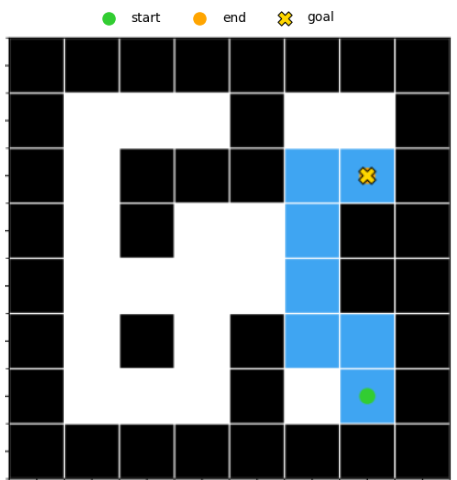
\includegraphics[width=1\linewidth]{example_trajectory.png}
	\captionsetup{font=small, justification=raggedright, singlelinecheck=false}
	\captionof{figure}{Example of a valid trajectory in a discrete 2D maze environment}
	\label{fig:example_trajectory}
\end{minipage}

\subsection{Approaches to Planning}

Reinforcement learning (RL) is a machine learning paradigm in which a system learns to choose
appropriate sequences of actions by interacting with an environment in order to maximise cumulative reward,
making it a natural fit for planning problems, since the reward can be defined in terms of 
reaching a goal state efficiently~\cite{sutton2018rl}.

Offline reinforcement learning is a variant of RL in which the policy that determines the agent's actions
is learned from a fixed dataset of previously collected trajectories, rather than through repeated
interaction with the environment~\cite{janner2021trajectory}.

Imitation learning is a related paradigm in which a model learns to reproduce the behaviour
demonstrated in a dataset. Similarly to offline RL, imitation learning can be applied to a dataset of 
trajectories, but the objective is to generate trajectories that are similar to those in the dataset,
as opposed to maximising cumulative reward as in offline RL~\cite{janner2021trajectory}.

Similarly to RL, imitation learning can solve a planning problem, but only if the dataset
contains trajectories that are valid and efficient for the planning task at hand~\cite{janner2021trajectory}.

In reinforcement learning, the term ``planning'' often refers to using a model of the environment to 
consider the likely consequences of possible actions before deciding which action to take. 
An important distinction must thus be made between
planning as a problem of generating a sequence of actions to reach a goal, and planning as a 
process of using a model to improve decision-making in reinforcement learning. In this 
work, the former interpretation is used.

\subsection{Generative Modelling for Planning}

If a dataset of valid trajectories is available, a generative model can be trained to learn the distribution over these trajectories. Once trained, the model can be used to generate new trajectories by sampling from the learned distribution. This approach treats planning as a problem of inference in a probabilistic model~\cite{janner2021trajectory}.
So if we define a trajectory $\boldsymbol{\tau}$ with $T$ steps as: 
\begin{equation}
\boldsymbol{\tau} = (s_1, a_1, s_2, a_2, \dots, s_T, a_T)
\end{equation}
where $s_t$ is the state (coordinates) at time step $t$ and $a_t$ is the action (moving up, down, left or right) taken at time step $t$, the trained generative model defines an approximation $p_{\hat{\boldsymbol{\theta}}}(\boldsymbol{\tau})$ to the distribution over valid trajectories.
Instead of directly modelling $p_{\hat{\boldsymbol{\theta}}}(\boldsymbol{\tau})$, an autoregressive model factorises this distribution into a product of conditional probabilities:
\begin{equation}
p_{\hat{\boldsymbol{\theta}}}(\boldsymbol{\tau}) = \prod_{t=1}^{T} p_{\hat{\boldsymbol{\theta}}}(z_t \mid z_{<t})
\label{eq:autoregressive_generative_model}
\end{equation}
where $z_t$ denotes the $t^{\text{th}}$ token in the flattened trajectory sequence, 
so each $z_t$ corresponds to either a single state token or a single action token, and 
the trajectory prefix, $z_{<t}$, denotes the sequence of preceding tokens up to $z_{t-1}$~\cite{goodfellow2016deep}.
This simplifies the supervised learning problem to estimating $p_{\boldsymbol{\theta}}(z_t \mid z_{<t})$, so given a prefix 
of trajectory tokens, predict the probability of the next token in the sequence. 

A complete trajectory is then generated autoregressively by repeatedly predicting the next token until a full plan is produced, with the decoding strategy determining how each next-token choice is made. The choice of decoding strategy is important because the model's predicted distribution may assign non-negligible probability mass to multiple valid continuations at each step, and the continuation selected during decoding can significantly affect both the quality of the final trajectory and the computational cost of generation~\cite{janner2021trajectory}. Since the learned distribution is only an approximation to the true trajectory distribution, it may also assign non-negligible probability to invalid continuations. As a result, the decoding strategy can influence whether a valid trajectory is generated at all. Even when multiple valid trajectories are possible, some may be more desirable than others, for example because they require fewer steps, and the decoding strategy can therefore affect whether a more efficient trajectory is produced~\cite{janner2021trajectory,jurafsky2026speech}.

\subsection{Decoding Methods}
Direct sampling from $p_{\hat{\boldsymbol{\theta}}}(\boldsymbol{\tau})$ is challenging, since the number of possible trajectories grows exponentially with trajectory
length, so explicitly calculating and storing the probabilities for all complete trajectories quickly  becomes computationally 
infeasible~\cite{goodfellow2016deep}. 
This creates a need for decoding algorithms to approximately sample from, or search within $p_{\hat{\boldsymbol{\theta}}}(\boldsymbol{\tau})$.



\subsubsection{Greedy Decoding}
Greedy decoding is the simplest method for generating sequences from $p_{\hat{\boldsymbol{\theta}}}(\boldsymbol{\tau})$~\cite{jurafsky2026speech}. 
At each step $t$ during the autoregressive generation of a trajectory, the algorithm selects the next token $\hat{z}_t$ 
as follows:
\begin{equation}
\hat{z}_t = \arg\max_{z \in V} p_{\hat{\boldsymbol{\theta}}}(z \mid z_{<t})
\end{equation}
where $V$ is the set of all possible tokens, and $z_{<t}$ denotes the values obtained in the previous steps of greedy decoding.
Greedy decoding thus always selects the locally optimal choice for the next token in the sequence, 
meaning it chooses the token with the highest conditional probability given
the current prefix~\cite{jurafsky2026speech}.
Greedy decoding is therefore deterministic and computationally efficient, but does not necessarily find the globally most probable 
trajectory, which is the complete trajectory with the highest probability under 
$p_{\hat{\boldsymbol{\theta}}}(\boldsymbol{\tau})$~\cite{jurafsky2026speech}.

\subsubsection{Beam Search}

Beam search extends greedy decoding by retaining multiple candidate sequences at each step rather 
than only the single most likely continuation~\cite{jurafsky2026speech}. The number of retained 
candidates is fixed in advance and is known as the beam width $B$. At each stage, all valid one-step 
continuations of the current candidates are scored autoregressively under the model, and the top $B$ 
highest-scoring sequences are kept. This process is repeated until termination, after which the 
highest-scoring complete trajectory among the retained candidates is returned.

The beam search algorithm used in this work is summarised in Listing~\ref{lst:beam_search_pseudocode}.

\begin{center}
\begin{minipage}{0.9\linewidth}
\begin{flushleft}
\hrule
\vspace{0.3em}
\textbf{Beam Search}~\cite{janner2021trajectory}
\vspace{0.3em}
\hrule
\vspace{0.6em}

\begin{tabular}{r p{0.82\textwidth}}
1: & \textbf{Require} maximum sequence length $T$, beam width $B$, starting position $s_{\mathrm{start}}$, and goal position $s_{\mathrm{goal}}$ \\[0.3em]
2: & \textbf{Initialize} $\mathcal{T}_0 = \{(s_{\mathrm{start}})\}$ \\[0.3em]
3: & \textbf{for} $t = 0, \dots, T-1$ \textbf{do} \\[0.3em]
4: & \hspace*{1.5em}For each partial trajectory $\boldsymbol{\tau} \in \mathcal{T}_t$, let $\mathcal{V}(\boldsymbol{\tau})$ denote the set of valid next tokens available from the final state of $\boldsymbol{\tau}$ \\[0.3em]
5: & \hspace*{1.5em}$C_{t+1} \leftarrow \{\, \mathrm{append}(\boldsymbol{\tau}, z) \mid \boldsymbol{\tau} \in \mathcal{T}_t \text{ and } z \in \mathcal{V}(\boldsymbol{\tau}) \,\}$ \\
   & \hspace*{1.5em}// candidate single-token extensions \\[0.3em]
6: & \hspace*{1.5em}$\mathcal{T}_{t+1} \leftarrow$ the set of the $B$ highest-scoring sequences in $C_{t+1}$ under $\log p_{\hat{\boldsymbol{\theta}}}(\boldsymbol{\tau})$ \\[0.3em]
7: & \hspace*{1.5em}\textbf{if} any $\boldsymbol{\tau} \in \mathcal{T}_{t+1}$ ends at $s_{\mathrm{goal}}$ \textbf{then stop} \\[0.3em]
8: & \textbf{end for} \\[0.3em]
9: & \textbf{Return} $\arg\max_{\boldsymbol{\tau} \in \mathcal{T}_{t+1}} \log p_{\hat{\boldsymbol{\theta}}}(\boldsymbol{\tau})$
\end{tabular}

\vspace{0.6em}
\hrule
\end{flushleft}
\end{minipage}
\captionsetup{type=lstlisting}
\captionof{lstlisting}{Pseudocode for beam search in the trajectory planning setting.}
\label{lst:beam_search_pseudocode}
\end{center}
Here, $t$ denotes the current decoding step, $\mathcal{T}_t$ the set of retained partial
trajectories at step $t$ and $C_t$ the corresponding set of candidate trajectories.
The score $\log p_{\hat{\boldsymbol{\theta}}}(\boldsymbol{\tau})$ can be accumulated autoregressively for each candidate trajectory. 
Since the beam width places an upper bound on the number of candidate trajectories in $C_t$ and retained trajectories in 
$\mathcal{T}_t$ at each step $t$, maintaining these scores for all candidates remains computationally 
feasible when the beam width is sufficiently small 
~\cite{jurafsky2026speech}.

Larger beam widths allow the algorithm to consider a greater number of candidate trajectories. As a result, 
the trajectory returned by beam search will typically be at least as highly scored under the model as the trajectory 
returned with a smaller beam width, with a beam width of one corresponding to greedy decoding. This broader search, however,
requires the model scores of more candidate trajectories to be computed and maintained, so increasing the beam width also 
increases the computational cost of decoding~\cite{jurafsky2026speech}.

Both greedy decoding and beam search, as defined above, aim to find trajectories with high probability
under the learned model, and therefore correspond naturally to an imitation learning setting. 
If, however, the decoding objective is defined in terms of predicted reward or return rather 
than model probability alone, then the same decoding procedures can instead be used in an 
offline reinforcement learning setting.


\subsection{Transformer Based Generative Models}

The Transformer is a type of neural network that has become the standard for sequence modelling tasks, notably in natural language processing~\cite{jurafsky2026speech}.
Even though the original Transformer was designed for language, the fact that it models sequences of tokens makes it applicable to our trajectory modelling problem, where the tokens could be states and/or actions in a trajectory~\cite{janner2021trajectory}.

The key components of the Transformer are now briefly introduced. For intuition, the discussion refers 
primarily to natural language processing examples, where the role of these components is often easier to 
interpret than in trajectory modelling. 

\textbf{1. Input Representation}

Before raw data enters the Transformer, it must be converted into a high dimensional vector representation
as follows.

\textbf{Tokenisation}


The first step involves tokenisation, where the input sequence is broken down into discrete tokens. In an NLP scenario, 
this could involve splitting text into words, subwords or characters~\cite{jurafsky2026speech}. For the purposes of this discussion, it is assumed that 
the input has been tokenised at the word level.

\textbf{Embeddings} ($E$) 

Each token ID is used to index into an embedding matrix $E$, which maps 
the discrete ID to a dense vector of dimensionality $d$. This matrix has shape $|V| \times d$, where $|V|$ is 
the vocabulary size, i.e.\ the total number of distinct tokens that the model can represent~\cite{jurafsky2026speech}.
When tokens correspond to words, the embedding can be interpreted as capturing semantic and syntactic properties of 
those words. Intuitively, words with similar meanings, such as ``big'' and ``large,'' may be represented by vectors 
that are close to one another in the embedding space~\cite{jurafsky2026speech}.

\textbf{Positional Encoding} 

Since the Transformer processes sequences in parallel, it does not 
inherently encode the order of tokens, so a positional encoding is added to the token embeddings to ensure that the 
position of each token in the sequence is represented. This is done by adding a positional encoding vector to each
token embedding~\cite{jurafsky2026speech}.

\textbf{Input Formation}

For a sequence of $N$ tokens, the individual $d$-dimensional vector embeddings are 
placed into a single matrix $X$ of size $N \times d$. This matrix serves as the input for the model~\cite{jurafsky2026speech}.

\textbf{2. Transformer Blocks}

Each block consists of a multi-head self-attention mechanism followed by a feedforward neural network, with each sublayer
followed by a layer normalisation and a residual connection~\cite{jurafsky2026speech}. 

A useful mental model is that each time the input passes through a sublayer, the model 
updates the token representations so that they better capture the information relevant to 
the task at hand. For example, in an NLP context, the model may refine the representation of a 
word so that it better reflects its meaning in the context of the sentence~\cite{jurafsky2026speech}.
Each block is described as follows.

\textbf{Layer Normalisation}

For training stability, layer normalisation is applied to ensure the values in the sublayers remain within a reasonable range.
For a vector $x$, it is calculated as:
\begin{equation}
\mathrm{LayerNorm}(x) = \gamma \odot \frac{x - \mu}{\sigma} + \beta
\end{equation}
where $\mu$ is the mean, $\sigma$ the standard deviation of the vector's elements, and $\gamma$ and $\beta$ are 
learned parameters that scale and shift the normalised output~\cite{jurafsky2026speech}.


\textbf{Multi-Head Self-Attention}

This is the core mechanism that allows the model to incorporate information from all tokens in the sequence
when processing each token~\cite{jurafsky2026speech}. Under the interpretation that each sublayer progressively 
refines word representations, the self-attention mechanism allows the representation of each word to be updated in 
light of the representations of all other words in the sequence. For example, if the word ``fly'' is preceded by the 
word ``the'', the model may adjust its representation in a way that reflects the nominal sense of ``fly'' (the insect)
rather than the verbal sense.
Each input vector $x_i$ is mapped into three learned representations: a Query ($Q$), a Key ($K$), and a Value ($V$).
For an input matrix $X$, these are obtained by learned linear projections:
\begin{equation}
Q = XW_Q,\qquad K = XW_K,\qquad V = XW_V
\end{equation}
where $W_Q$, $W_K$, and $W_V$ are learned weight matrices~\cite{jurafsky2026speech}.

The attention for a single head is computed as:
\begin{equation}
\mathrm{Attention}(Q, K, V) = \mathrm{softmax}\left(\frac{QK^T}{\sqrt{d_k}}\right)V
\end{equation}

The scaling factor $\sqrt{d_k}$ prevents the dot products from growing too large and causing numerical 
instability. In causal (left-to-right) models, such as predicting the next word in a sentence, or the next position
in a trajectory, a mask is applied to ensure that tokens can only attend to the 
past, preventing the model from ``cheating'' by looking at future tokens during training~\cite{jurafsky2026speech}.

\textbf{Feedforward Neural Network}

After the attention layer incorporates information across tokens, the Feedforward Network (FFN) processes each token position 
independently and in parallel~\cite{jurafsky2026speech}. It is usually a two-layer network with a non-linear activation such as ReLU:
\begin{equation}
\mathrm{FFN}(x) = \mathrm{ReLU}(xW_1 + b_1)W_2 + b_2
\end{equation}
This layer allows the model to perform more complex transformations of the contextualised information
gathered by the attention heads~\cite{jurafsky2026speech}. 

Returning to the intuitive picture introduced earlier, the attention mechanism can be viewed as first 
updating each word representation using information from the other words in the sequence. The FFN then 
further refines each of these updated representations independently at each position, using transformations 
learned from many training sequences.

\textbf{3. Prediction Head}

After the data passes through the final transformer block, the final representations are passed 
to the next-token prediction head, which converts them into a probability distribution over possible next 
tokens in the sequence. This is done through the following steps.

\textbf{Output Projection} 


Let $\mathbf{h}_t$ denote the final hidden representation produced after
the model has processed the prefix up to position $t$. This $d$-dimensional vector summarises the
information in the observed prefix and is then projected back into the vocabulary space, often by
multiplying it by the transpose of the embedding matrix $E^T$~\cite{jurafsky2026speech}.

\textbf{Softmax}

The resulting logits are passed through a softmax function to produce a 
probability distribution over the next token:
\begin{equation}
\mathbf{p}_{t+1} = \mathrm{softmax}(\mathbf{h}_t E^T)
\end{equation}

where $\mathbf{p}_{t+1}$ is the probability distribution over possible values of the next token
$z_{t+1}$ given the prefix $z_{\le t}$~\cite{jurafsky2026speech}.

In general, this means that the model assigns a probability to each possible next token given the preceding 
trajectory prefix. In an NLP setting, where tokens correspond to words, this can be interpreted as the model 
estimating which word is most likely to come next in the sentence. The next token is then selected according 
to a decoding strategy such as greedy decoding, sampling, or beam search.

\subsection{The Markov Property}

In planning tasks, there is typically an environment state that evolves over time as
actions are taken. The Markov property states that the probability distribution of the
next state depends only on the current state and the action taken, and not on the history
of states and actions that led to the current state~\cite{sutton2018rl}. In the previously
discussed problem of finding a sequence of actions connecting a starting position to a
goal position in a known maze, the Markov property holds if the current position, selected
action, and maze layout are sufficient to determine the probability distribution over
possible next positions.

If the maze layout is known and constant, and $(s_1,s_2,\dots,s_t)$ are successive
positions in the maze, then the state-transition process satisfies the Markov property if
\begin{equation}
p(s_t \mid s_1,a_1,s_2,a_2,\dots,s_{t-1},a_{t-1})
=
p(s_t \mid s_{t-1},a_{t-1}).
\label{eq:markovian_maze}
\end{equation}

If the next position is uniquely determined by the current position and selected action,
then there exists a transition function $f$ such that
\begin{equation}
s_t=f(s_{t-1},a_{t-1}).
\end{equation}
The maze environment therefore has deterministic Markovian transition dynamics.

If the objective is to train a generative model that estimates a probability
distribution over possible next actions for maze planning, it may be
advantageous to condition the model on all previous states and actions. The
model therefore predicts
\begin{equation}
p(a_t \mid m,s_{\mathrm{start}},s_{\mathrm{goal}},
s_1,a_1,s_2,a_2,\dots,a_{t-1},s_t)
\end{equation}
rather than
\begin{equation}
p(a_t \mid m,s_{\mathrm{start}},s_{\mathrm{goal}},s_t),
\end{equation}
even if the state-transition process satisfies
Equation~\eqref{eq:markovian_maze}.

The hypothesis is that previous states and actions can still provide useful
information to the model when predicting the probability distribution over
next actions. For example, if the model returns to a position that it has
already visited, the trajectory prefix allows it to identify the earlier visit
and may help it avoid repeating the same sequence of actions. The key
distinction is that the Markov property describes the environment's transition
dynamics, rather than the information on which a learned model may be
conditioned. The fact that the next state is determined by the current state
and selected action therefore does not prevent a learned sequence model from
using previous states and actions when predicting the next-action distribution.


\subsection{Partially Observed States}

The Markov property is a property of an environment or stochastic process. An agent navigating the 
environment, or a model predicting aspects of it, may assume that the Markov property holds. 
Under this assumption, the probability distribution of the next state depends only on the 
current state and selected action, rather than on the complete history of previous states and 
actions. If the complete current state and the environment’s transition dynamics are known, the 
probability distribution of the next state after taking a particular action can be calculated. In practice, 
however, an agent or model may not have access to the complete state of the environment. Instead, only
certain parts or aspects of that state may be observed. In this case, the environment is said to be
partially observed from the perspective of the agent or model.

In the context of the maze planning problem, the maze layout being known implies that 
coordinates of the current position provide
enough information to know the exact position within the maze. If the
model is however not provided with its exact coordinates in a maze,
but rather with a local view of the maze layout, such as a 3x3 grid of cells 
surrounding the current position, then the model does not have enough information 
to know its exact position in the maze, as multiple positions in multiple maze 
layouts may correspond to the same local view. These local views
are denoted as observations $(\mathbf{o}_1,\mathbf{o}_2,\dots,\mathbf{o}_t)$, 
and are provided to the model instead of the exact states. When the complete
states are not made available to the model, the states are said to be partially observed.
The environment can still be Markovian, but the current pbservation and action may not 
provide enough information to determine the next observation, so the observation 
process may not satisfy the Markov property. A model may need to rely on 
previous observations and actions to infer its current position in the maze.



\section{Research Questions}

The objective of this work is to compare different decoding strategies when 
modelling maze planning as autoregressive inference in a learned conditional 
trajectory model trained through next-token prediction. The performance of 
greedy decoding and beam search with different beam widths are evaluated in terms of 
trajectory validity, goal-reaching success, path efficiency, and computational cost.

The decoding strategies are compared under different representations of the environment.
The first experiment is conducted in a discrete maze environment, where the maze
layout as well as the exact coordinates of the goal position, starting position and subsequent
states are provided. Decoding algorithms are thus evaluated in a fully observable setting, where the 
model has access to all relevant information about the environment.

The second experiment utilises the same maze layouts and training trajectories as the
first, but the model is not provided with the maze layout or the exact coordinates of 
the goal position. The model is instead provided with the relative direction of the 
goal position, and a layout of the 3x3 grid surrounding the current position istead of the 
complete states.
This formulation is therefore a partially observable setting, and the model will 
need to rely on previously observed trajectory information to infer unobserved 
information about the maze layout.

\section{Fully Observed Planning}

\subsection{Problem Formulation}

The objective of this experiment is to evaluate different decoding strategies
by training a conditional trajectory model through next-token prediction in a fully
observed maze environment.
Given a maze layout identifier, a start state, a goal state, and a trajectory prefix consisting
of previous actions and explicit coordinates of previous states in the maze, the model 
predicts the next action in the trajectory sequence. At inference time, decoding algorithms are
then used to construct complete trajectories by selecting continuations with high probability 
under the learned model. Since decoding is based on model probability rather than a reward-maximising 
objective, this amounts to using imitation learning to solve the planning problem.

A trajectory $\boldsymbol{\tau} = (z_1, z_2, \dots, z_{2T})$ consists of alternating state and action 
tokens, \\ $(s_1, a_1, s_2, a_2, \dots, s_T, a_T)$, where the states represent coordinates in the maze and 
the actions correspond to the moves (up, down, left, or right) between consecutive states. In this 
environment, the state immediately following an action is fully determined by that action and the 
preceding state. Supervision is therefore applied only at action-token positions, so the learning problem 
is more precisely to predict the next action conditioned on the maze layout, the start state, the goal 
state, and the previously observed trajectory prefix.

Let $m$ denote a maze layout identifier, let $s_{\mathrm{start}}$ and $s_{\mathrm{goal}}$ denote the start and goal states. 
The model therefore learns conditional predictions of the form

\begin{equation}
p_{\hat{\boldsymbol{\theta}}}(a_{t} \mid m, s_{\mathrm{start}}, s_{\mathrm{goal}}, s_1, a_1, \dots, s_t),
\end{equation}

These conditional predictions define an autoregressive factorisation of the 
conditional distribution over action sequences:

\begin{equation}
p_{\hat{\boldsymbol{\theta}}}(a_1, a_2, \dots, a_T \mid m, s_{\mathrm{start}}, s_{\mathrm{goal}})
=
\prod_{t=1}^{T}
p_{\hat{\boldsymbol{\theta}}}(a_t \mid m, s_{\mathrm{start}}, s_{\mathrm{goal}}, s_1, a_1, \dots, s_t).
\end{equation}

Ideally, generating a complete plan would require sampling from the full joint conditional
distribution over actions and observations above; in practice, the decoding algorithms instead operate on
its autoregressive conditional factors.



A Transformer was selected as the generative model because of its demonstrated
performance on sequence-modelling tasks~\cite{vaswani2017attention},
the wide range of Python libraries available for working with it, and its computational efficiency when the architecture is 
kept small. The research question, however, is not whether a Transformer can represent such a distribution in principle, but
how different decoding strategies affect the quality of the generated plans once the model has been trained.
In particular, the methodology compares the performance of greedy decoding and beam search in a fully observed  maze environment.
The performance is measured in terms of trajectory validity, goal-reaching success,
path efficiency, and computational cost.


\subsection{Methodology}

\subsubsection{Dataset Construction}

A trajectory token 
sequence provides multiple supervised training examples, since for each token position $k$
in a given trajectory, the prefix
\begin{equation}
(z_1, z_2, \dots, z_{k-1})
\end{equation}
can be used to predict the next token $z_k$.
In addition to the trajectory tokens themselves, the model input must encode which maze the trajectory 
belongs to, as well as the associated start and goal positions.

This work considers eight maze layouts from the D4RL PointMaze/Maze2D
environment. The exact layout definitions are provided in the D4RL repository's
\texttt{maze\_model.py} file~\cite{d4rlrepo}. Figure~\ref{fig:maze_layouts} shows
the eight layouts, which vary in size and structural complexity. This variation
allows the decoding strategies to be evaluated across a range of planning
problems.


\begin{figure}[H]
	\centering
	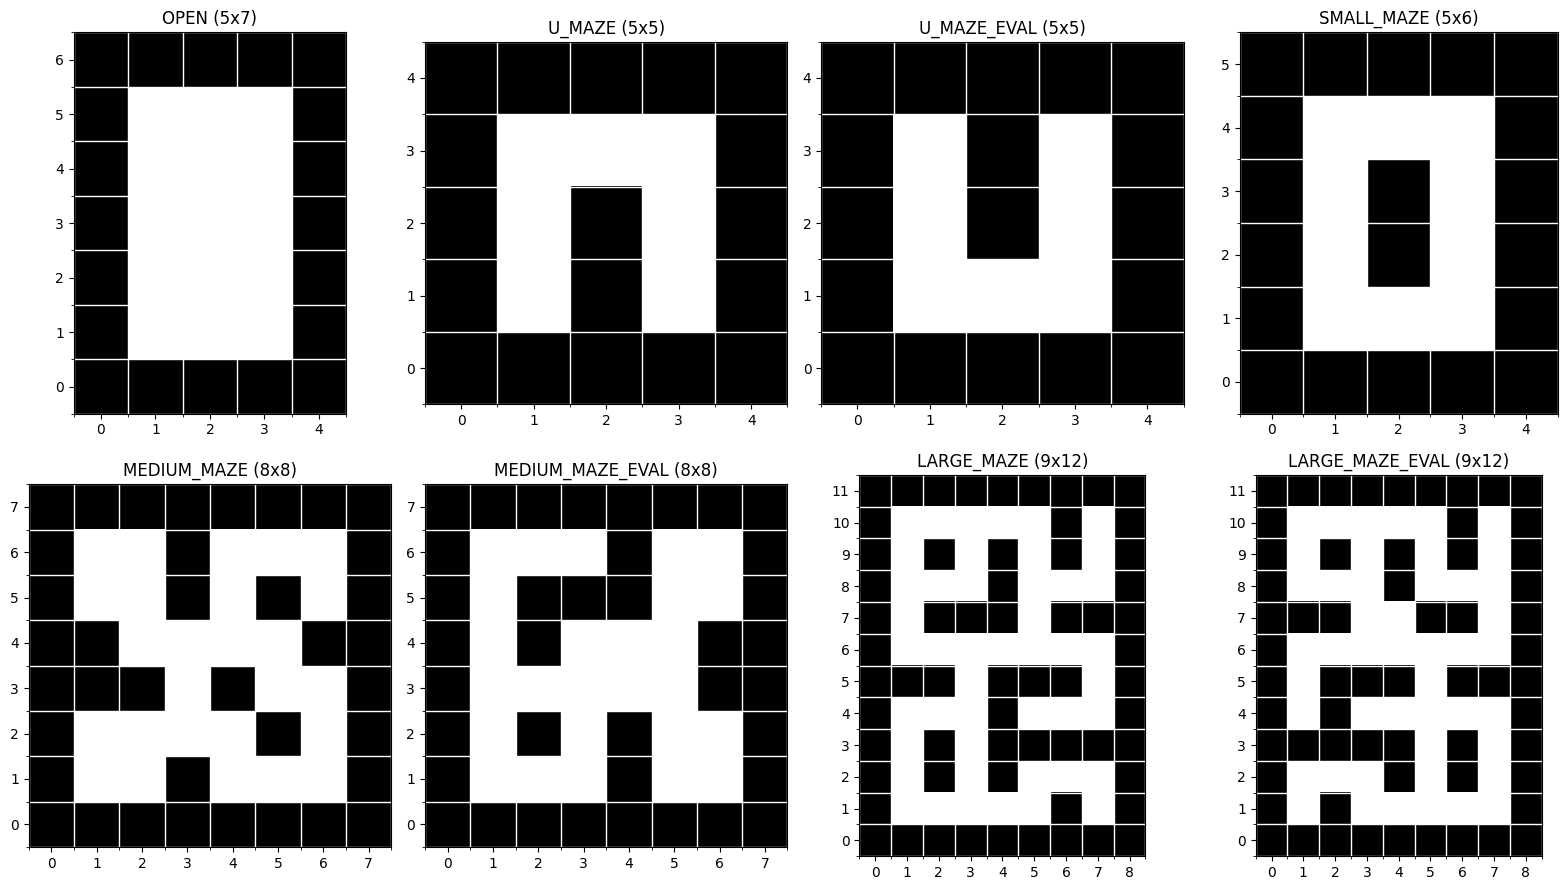
\includegraphics[width=0.9\textwidth]{maze_layouts.png}
	\caption{Maze layouts used from the D4RL PointMaze / Maze2D environment.}
	\label{fig:maze_layouts}
\end{figure}

Each maze is defined as a matrix, 
and the row and column indices of this matrix determine the corresponding grid cells in 
the discrete maze representations used throughout this work.

To represent the states, actions, and maze layouts as Transformer inputs, 
each is encoded as a discrete integer token. Distinct token ranges are reserved for 
different token classes by defining token offsets, so that maze tokens, state tokens, and action 
tokens occupy non-overlapping regions of the overall vocabulary.

States are encoded by assigning each grid location a unique integer index. This is done using the
mapping
\begin{equation}
\text{state\_index} = \text{row} \times (\text{max columns}) + \text{column},
\end{equation}
where \textit{row} and \textit{column} are the integer indices of the grid location, 
and \textit{max columns} is the maximum number of columns across all maze layouts. This 
produces a unique integer identifier for each location in the global grid. A state token 
is then obtained by adding a fixed state-token offset to this index. Although this indexing 
scheme assigns identifiers to all grid locations in the global grid, including wall locations, 
only valid free-cell positions appear in the generated trajectory sequences.

Actions are also encoded as integer tokens. Since the trajectories are restricted to 
four-connected grid movements, the action vocabulary consists of the four moves up, down, 
left, or right, with each assigned its own unique integer token identifier.

In the training data, the detailed wall structure of a maze is not included explicitly
in the token sequence. Instead, each trajectory is associated with a single integer maze token
identifying which of the eight layouts it belongs to. The model must infer the relevant layout 
constraints from this maze identifier together with the observed trajectory tokens. This design
choice gives a simple and efficient encoding scheme, but it also means that the model is tied 
to the set of maze layouts seen during training and cannot directly generalise to previously 
unseen layouts without additional representation of maze geometry.

The tokenised input sequences are stored in an input matrix $X$ of dimensions $N \times L$, 
where $N$ is the number of training trajectories and $L$ is the maximum token-sequence length 
observed in the training dataset.

The final form of each row $\boldsymbol{x}$ of the input matrix $X$ is
\begin{equation}
\boldsymbol{x}
=
(
m,\,
s_{\mathrm{start}},\,
s_{\mathrm{goal}},\,
s_1,\,
a_1,\,
s_2,\,
a_2,\,
s_3,\,
\dots,\,
a_T,\,
s_{T+1},\,
0,\,
\dots,\,
0
).
\end{equation}

where $s_{\mathrm{start}}$ and $s_{\mathrm{goal}}$ are represented using the same coordinate encoding 
as the states appearing in the trajectory. The sequence $(s_1, a_1, s_2, a_2, \dots, s_T, a_T)$ 
represents the alternating state and action tokens that make up the trajectory. Any unused entries 
at the end of the row are filled with padding tokens (0) so that all rows of $X$ have the same length.

For each maze layout, every valid ordered pair of distinct, non-wall start and
goal positions was considered. Breadth-first search (BFS) was used to find a
shortest path connecting each pair. The positions along each resulting path,
together with the actions corresponding to the movements between consecutive
positions, were stored as complete state-action trajectories for training the
Transformer. 

To compare decoding strategies on unseen queries, the transformer-ready dataset is partitioned using
5-fold cross-validation. The dataset contains exactly one trajectory for each ordered start-goal pair
that is connected by a valid shortest path in a given maze. Within each maze, trajectories were 
ordered lexicographically by path length,
start row, start column, goal row, and goal column. They were then assigned to
the five folds in round-robin order: the first trajectory was assigned to fold
1, the second to fold 2, and so on, returning to fold 1 after every fifth
trajectory. This deterministic
procedure was chosen to make the cross-validation split reproducible. Because each
start-goal pair appears only once in the dataset, no exact query appears in both the training and
evaluation portions of a given fold. In the decoding benchmark, evaluation is reported on the eight
maze families as seen in Figure~\ref{fig:maze_layouts}. The aim of the experiment is therefore to compare how different decoding 
rules behave on unseen start-goal planning queries under a fixed trained model class. 

\subsubsection{Transformer Training}

In addition to the input matrix $X$,
the token-type information is stored in a token-type matrix $T$, 
the target outputs are stored in a label matrix $Y$, and 
the padding information is stored in a mask matrix $M$. $T$, $Y$ and $M$ are all of the same shape as $X$.
Each entry in the token-type matrix indicates whether the corresponding token is a maze token, start token, goal token, 
state token, action token, or padding token. In the label matrix, only action-token positions contain 
active targets, while all other positions are ignored during loss computation. 
The mask matrix indicates which positions in the input sequences are padding tokens.

A small causal Transformer was trained on the tokenised trajectory datasets. 
After the model receives the training data, 
token embeddings and token-type embeddings are summed, positional encodings
are added, and the resulting sequence is processed by a stack of causal self-attention layers so that
each token can depend only on the current and preceding tokens in the sequence.

The model was kept small for faster training. The architecture used a hidden dimension of 64, 4 attention 
heads, 2 Transformer layers, a feedforward dimension of 128, and dropout of 0.1. Training was performed using the 
AdamW optimiser with learning rate $3 \times 10^{-4}$ and weight decay $10^{-4}$. For each training fold,
the model was trained for 20 epochs on the training partition of the fold, with a batch size of 128.
After every epoch, the model was evaluated on both the training and validation partitions of the fold.
The checkpoint with the best validation loss was saved and used for decoding evaluation.

The training objective was cross-entropy loss applied to next-token prediction, 
with supervision active only at action-token positions. This corresponds to modelling each 
conditional action distribution as categorical over a finite vocabulary, for which cross-entropy 
is the negative log-likelihood objective. Non-action positions in the 
label matrix $Y$ were ignored during loss computation.

\subsubsection{Decoding}

The decoding strategies compared in this work are greedy decoding and beam search with beam widths
$2$ and $3$. The trained Transformer predicts a distribution over the next action token conditioned
on the maze token, start token, goal token, and the trajectory prefix generated so far. Decoding
then determines how these conditional predictions are converted into a complete trajectory.

For a given evaluation query, decoding begins from the token prefix consisting of the maze
identifier, the start token, the goal token, and the initial state token. The model is
then queried autoregressively for the next action token. In the implementation used here, the model's
logits are not accepted blindly over the full action vocabulary. Instead, at each step, the candidate
actions are restricted to the actions that lead to valid neighbouring free cells from the current
state. In other words, candidate moves that
would pass through walls or leave the maze are excluded before the decoding rule is applied. Once an
action has been selected, the corresponding next state is deterministically computed from the current
state and appended to the trajectory prefix, and the procedure repeats until the goal is reached or a
step limit is exceeded.

The step limit refers to the maximum number of decoding steps, equivalently the maximum number of 
action predictions, that a decoding algorithm is allowed to generate for a query before termination 
is forced if the goal has not yet been reached. In the implementation used here, this limit is fixed 
at $19$ steps for all queries. This value was chosen as it is the maximum number of actions to reach the 
goal found in the training dataset across all maze layouts.

\subsubsection{Evaluation Metrics}


Since the Transformer only provides an
estimated conditional distribution over next actions, a decoding strategy may fail to reach the goal
within the allowed horizon even when a valid path exists. For this reason, the first evaluation
metric is \textbf{Completion Rate}, defined as the proportion of evaluation queries for which the
decoded trajectory reaches the goal within the allowed number of steps.

The second metric is \textbf{Average Steps to Goal}. In the implementation, this is computed as the
mean number of executed actions, equivalently the number of state transitions, over successful
queries only. This metric measures the efficiency of the trajectories produced by a decoding
strategy, conditional on success.	

The remaining two metrics quantify computational cost. For each decoded trajectory, the total wall-clock
time required to perform decoding is recorded. This yields \textbf{Average Compute Seconds}, defined
as the mean total decoding time per evaluation query. In addition, the total decoding time for a
query is divided by the number of decoded actions taken for that query, yielding a per-query seconds
per step quantity. Averaging this value over evaluation queries gives \textbf{Average Seconds per
Step}. Together, these four metrics allow the comparison to capture both planning quality and
computational efficiency.

\subsection{Results and Discussion}

Table~\ref{tab:completion_rate_all8} and Table~\ref{tab:avg_steps_all8} report decoding performance across the eight maze layouts, aggregated over the
full cross-validation evaluation. The main text focuses on completion rate and average steps to goal.
The full set of results, including completion rate, average steps to goal, average compute time, and average 
time per step, is reported in Appendix~\ref{app:per_maze_results}.

\begin{table}[H]
\centering
\caption{Completion rate across all eight maze layouts.}
\label{tab:completion_rate_all8}
\footnotesize
\begin{tabular}{lccc}
\hline
Maze Layout & Greedy & Beam 2 & Beam 3 \\
\hline
OPEN & 0.8292 & 0.9500 & 0.9958 \\
U\_MAZE & 0.7333 & 0.9778 & 1.0000 \\
U\_MAZE\_EVAL & 0.8667 & 1.0000 & 1.0000 \\
SMALL\_MAZE & 1.0000 & 1.0000 & 1.0000 \\
MEDIUM\_MAZE & 0.7492 & 0.9338 & 0.9892 \\
MEDIUM\_MAZE\_EVAL & 0.6292 & 0.9015 & 0.9677 \\
LARGE\_MAZE & 0.6657 & 0.9092 & 0.9850 \\
LARGE\_MAZE\_EVAL & 0.6901 & 0.8941 & 0.9598 \\
\hline
\end{tabular}
\normalsize
\end{table}

\begin{table}[H]
\centering
\caption{Average steps to goal across all eight maze layouts.}
\label{tab:avg_steps_all8}
\footnotesize
\begin{tabular}{lccc}
\hline
Maze Layout & Greedy & Beam 2 & Beam 3 \\
\hline
OPEN & 5.7839 & 3.9825 & 3.3724 \\
U\_MAZE & 4.0152 & 3.7159 & 3.6889 \\
U\_MAZE\_EVAL & 4.3718 & 3.6667 & 3.6667 \\
SMALL\_MAZE & 2.2500 & 1.6667 & 1.6667 \\
MEDIUM\_MAZE & 6.4784 & 5.3674 & 5.2022 \\
MEDIUM\_MAZE\_EVAL & 6.0513 & 5.3737 & 5.1669 \\
LARGE\_MAZE & 8.6016 & 8.1722 & 7.9971 \\
LARGE\_MAZE\_EVAL & 8.4551 & 7.8081 & 7.6361 \\
\hline
\end{tabular}
\normalsize
\end{table}


It is observed in Tables~\ref{tab:completion_rate_all8} and~\ref{tab:avg_steps_all8} that beam
search with width $B=2$ and $B=3$ outperforms greedy decoding in terms of both completion rate and average steps to goal,
with the larger beam width yielding the best overall performance. This is consistent with the
expectation that a broader search over candidate trajectories yields trajectories with higher
probability under the learned model, and since the model was trained on optimal trajectories,
these higher-probability trajectories are more likely to correspond to valid and efficient paths
to the goal.

The trade-off typically associated with beam search, relative to greedy decoding, and with
increasing beam width, is that the broader search requires more computation. In the aggregate, the
average time per step is indeed higher for beam search than for greedy decoding, and it also
increases with beam width. However, in this
implementation the average total compute time per query as reported in Appendix~\ref{app:per_maze_results} 
is lower for beam search than for greedy
decoding, and is also lower for $B=3$ than for $B=2$. This can be explained by the fact that
broader searches reach the goal in fewer steps on average, so the reduction in the number of
decoded steps outweighs the increase in time per step, yielding a lower total compute time.

The performance of the decoding strategies did vary across maze layouts, as reported in
Appendix~\ref{app:per_maze_results}. However, the relative ordering in completion rate and average
steps to goal was consistent across all maze layouts: beam search performed at least as well as
greedy decoding, and $B=3$ performed at least as well as $B=2$. For average time per step, the same overall pattern also
held in almost all cases. The only exception was the U\_MAZE layout, where beam search with width
$B=3$ had a slightly lower average time per step than beam search with width $B=2$.

In some mazes, the average total compute time did not decrease monotonically with beam width. This
occurred in layouts where there were typically fewer valid path options from a given state, so the
average steps to goal of the broader searches were close to, or equal to, those of the narrower
searches. In those cases, the additional per-step cost of the broader search was not always offset
by a shorter decoded trajectory.

\section{Partially Observed Planning}

\subsection{Problem Formulation}

The objective of this experiment is to evaluate different decoding strategies for a
conditional trajectory model trained through next-token prediction under a partially
observed setting. At each time step, the model is
provided with neither the maze layout nor the absolute coordinates of the agent or goal.
Instead, it receives a $3\times3$ grid of cells centred on its current position and the
displacement of the goal relative to that position. The relative displacement provides
the row and column offsets of the goal, including their directions, without revealing the agent's
absolute position or the unobserved maze layout. It does not provide the shortest-path
distance through the maze.

Unlike in the fully observed experiment, where the complete maze layout is available,
the preceding trajectory tokens now contain information that may not be present in the
current local observation. Figure~\ref{fig:true_state_vs_partial_observation} contrasts
the complete maze layout and the agent's position with the local observation at a given
time step. The right panel represents all the information supplied
to the model at that time step. In this partially observed setting, a planning algorithm 
does not have access to the true observations that would follow a sequence of actions without 
executing those actions in the environment. The planner can still compare possible future
trajectories, but it must construct them using the trajectory information available so far 
and the model’s predicted observations rather than the true future observations. 
This restriction did not arise in the fully observed experiment because the complete maze 
layout and deterministic movements made it possible to calculate the exact sequence of states 
resulting from any candidate action sequence without executing it in the environment.

Conditioning on the complete
trajectory prefix allows the Transformer to use previous observations and actions to
infer unobserved aspects of the maze layout. The partially observed setting therefore
allows the decoding strategies to be compared in a problem where an advantage of the
Transformer-based sequence-modelling framework is particularly relevant: its ability to
use trajectory context when the current observation alone is insufficient for selecting
the next action.

At inference time, the same decoding algorithms as in the previous experiment are
used to construct complete trajectories by selecting continuations with high probability
under the learned model. As in the previous experiment, the model is trained by
imitating demonstrated trajectories, and decoding is based on model probability rather
than reward maximisation. The action-selection component therefore remains based on
imitation learning, while observation prediction allows beam search to evaluate imagined
continuations, which refer to predicted values of unknown future observations that 
would follow candidate action sequences.

During decoding, beam search needs to form a set of candidate trajectories. In the previous experiment,
beam search could calculate the exact trajectories corresponding to each candidate action sequence, 
since the exact position in the maze after every action is known. In the partially observed setting, however,
the observations that would follow hypothetical actions are not known, so they must be
predicted.
Supervision during training is thus applied to the observations as well as the actions in 
the sequences. 

Let $o_t$ denote the local observation at time step $t$, consisting of the $3\times3$
grid of cells surrounding the agent's current position. The position of the goal is
provided separately as the relative displacement
\begin{equation}
\Delta \mathbf{g}_t
=
\begin{pmatrix}
r_{\mathrm{goal}}-r_t \\
c_{\mathrm{goal}}-c_t
\end{pmatrix},
\end{equation}
where $(r_t,c_t)$ denotes the agent's current position and
$(r_{\mathrm{goal}},c_{\mathrm{goal}})$ denotes the goal position. For notational
convenience, the complete observation supplied at time step $t$ is denoted by
\begin{equation}
\mathbf{y}_t=(o_t,\Delta \mathbf{g}_t).
\end{equation}

A trajectory containing $T$ observations therefore has the form
\begin{equation}
\boldsymbol{\tau}
=
(\mathbf{y}_1,a_1,\mathbf{y}_2,a_2,\dots,
\mathbf{y}_{T-1},a_{T-1},\mathbf{y}_T),
\end{equation}
where each action $a_t$ is one of the four movements (up, down, left, or right)
performed between observations $\mathbf{y}_t$ and $\mathbf{y}_{t+1}$. The model is
not provided with a maze identifier, the complete maze layout, or the absolute
coordinates of the agent or goal.

The first observation $\mathbf{y}_1$ is supplied to the model. Supervision is then
applied to each action and each post-action observation. The model consequently learns
conditional predictions of the forms
\begin{equation}
p_{\hat{\boldsymbol{\theta}}}
(a_t \mid \mathbf{y}_1,a_1,\mathbf{y}_2,a_2,\dots,
a_{t-1},\mathbf{y}_t),
\end{equation}
and
\begin{equation}
p_{\hat{\boldsymbol{\theta}}}
(\mathbf{y}_{t+1} \mid \mathbf{y}_1,a_1,\mathbf{y}_2,a_2,\dots,
\mathbf{y}_t,a_t).
\end{equation}
Since $\mathbf{y}_{t+1}$ is represented by multiple tokens, its components are
themselves predicted autoregressively in their token order.

These conditional predictions define an autoregressive factorisation of the joint
conditional distribution over future actions and observations:
\begin{equation}
\begin{split}
&p_{\hat{\boldsymbol{\theta}}}
(a_1,\mathbf{y}_2,a_2,\dots,a_{T-1},\mathbf{y}_T
\mid \mathbf{y}_1) \\
&\quad =
\prod_{t=1}^{T-1}
p_{\hat{\boldsymbol{\theta}}}
(a_t \mid \mathbf{y}_1,a_1,\dots,a_{t-1},\mathbf{y}_t)
p_{\hat{\boldsymbol{\theta}}}
(\mathbf{y}_{t+1} \mid \mathbf{y}_1,a_1,\dots,\mathbf{y}_t,a_t).
\end{split}
\end{equation}


\begin{figure}[H]
	\centering
	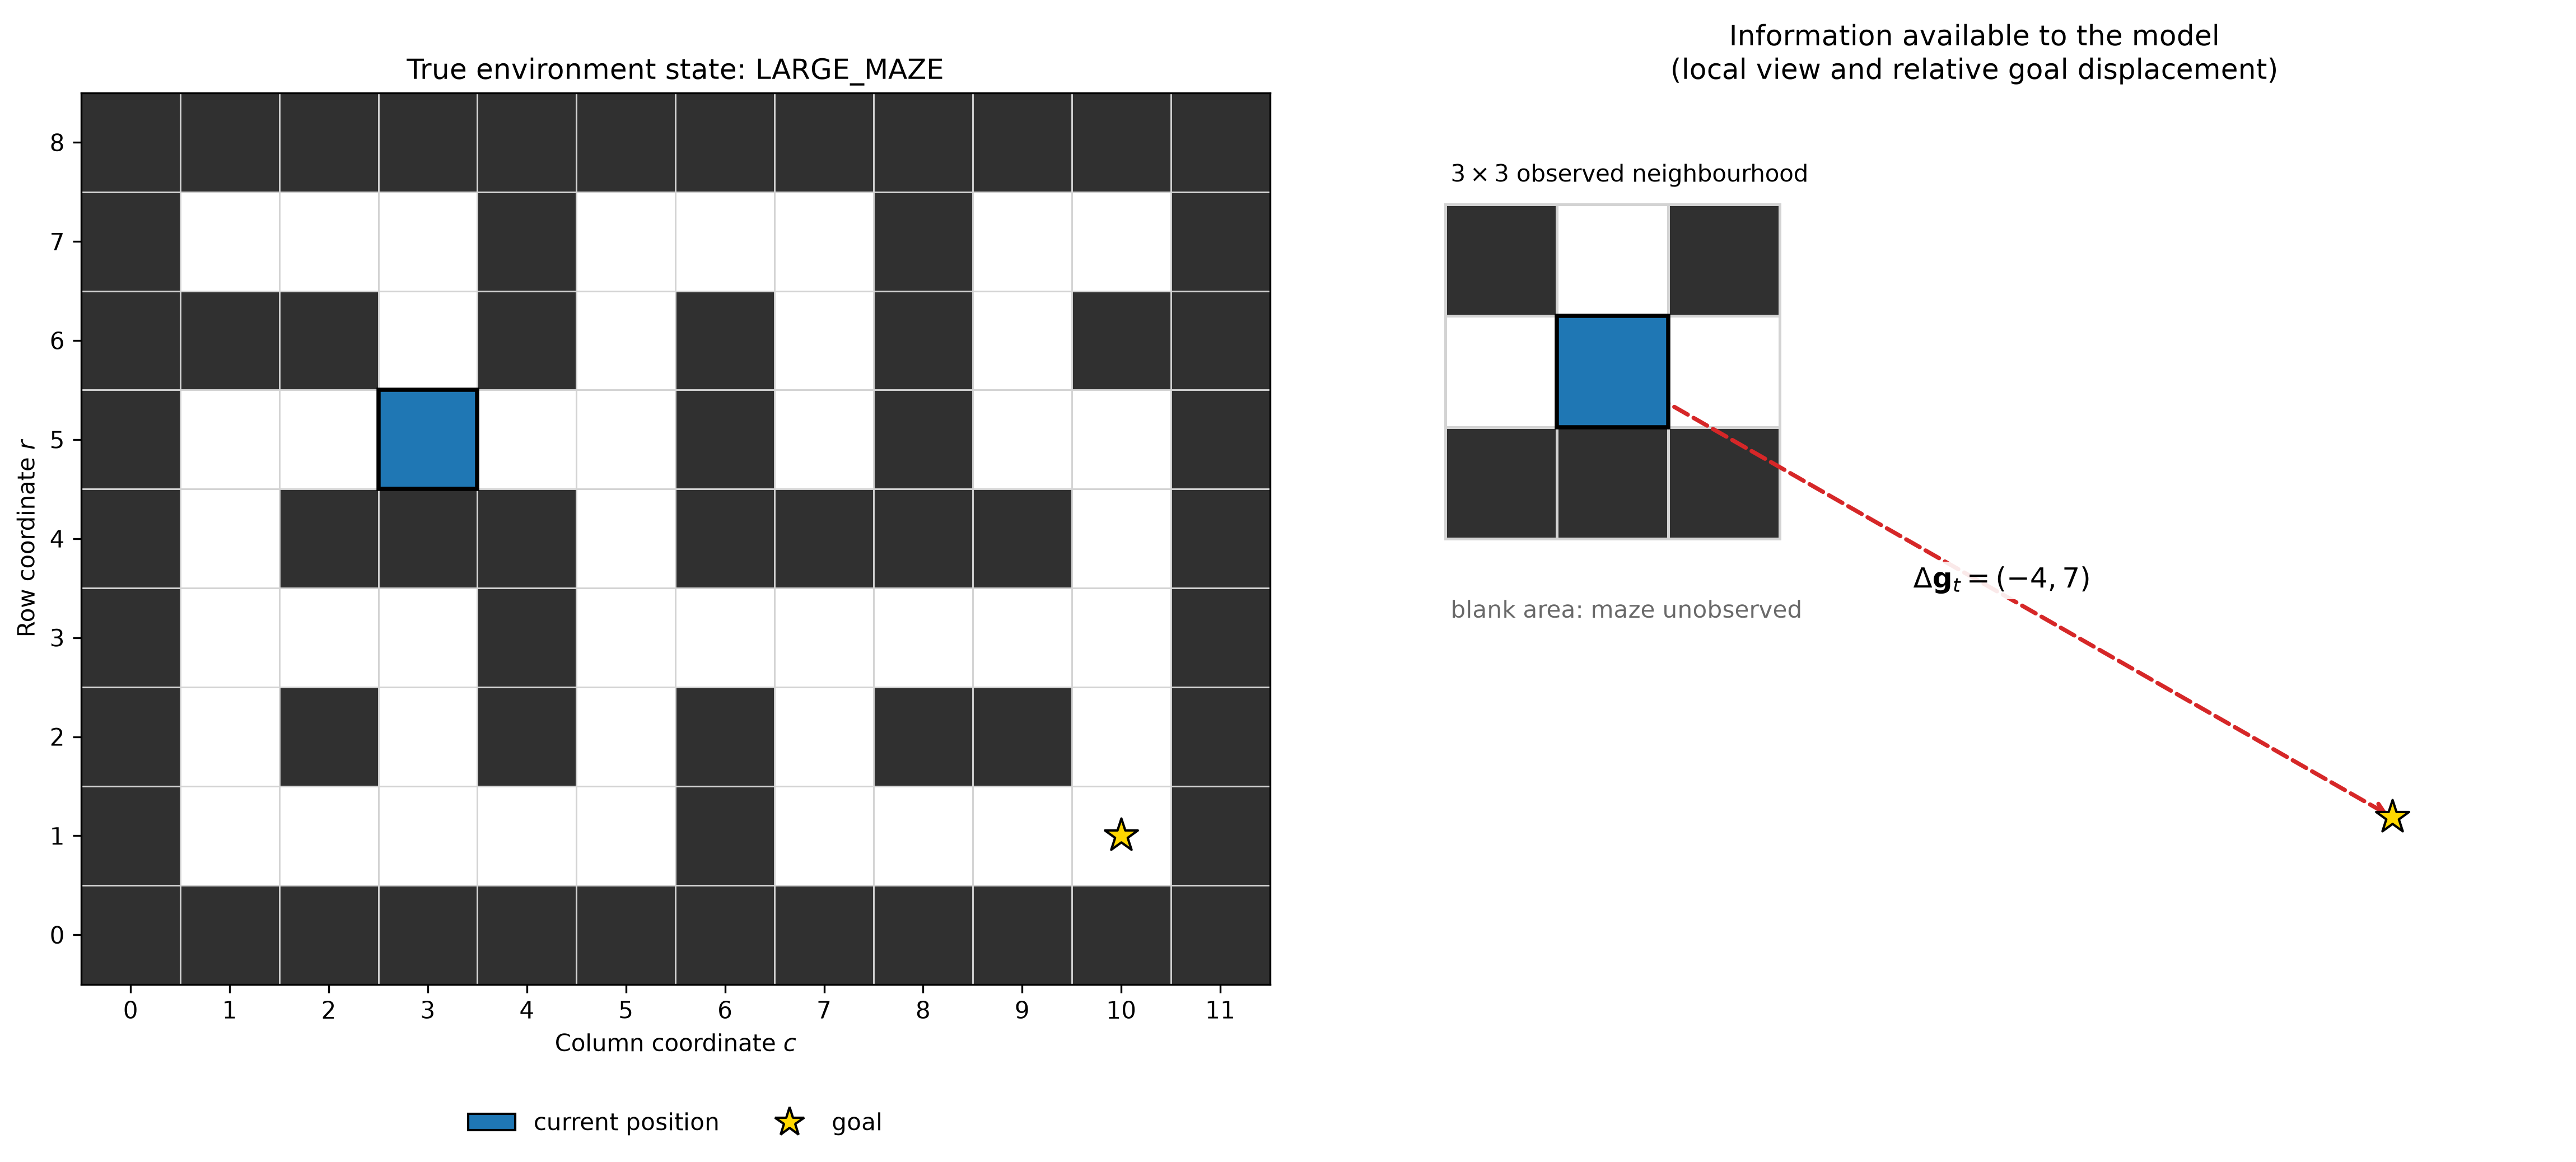
\includegraphics[width=\textwidth]{partial_observation_vs_true_state.png}
	\caption{Comparison of the true maze state and the corresponding partial observation at the same time step. The left panel shows the full
	\texttt{LARGE\_MAZE} layout, the agent's current position, and the goal using
	absolute grid coordinates. The right panel shows only the local $3\times3$
	neighbourhood and the goal's relative displacement.}
	\label{fig:true_state_vs_partial_observation}
\end{figure}


\subsection{Methodology}

\subsubsection{Dataset Construction}

The partially observed dataset is constructed from the same eight mazes and the same
optimal BFS trajectories as the fully observed dataset. The ordered start-goal queries,
action sequences, path lengths, episode identifiers, maze assignments, and five-fold
split assignments are retained unchanged. The trajectories are therefore not generated
again; instead, the fully observed state representation is replaced by the partial
observation representation defined above. This preserves a controlled comparison between
the experiments while avoiding repetition of the trajectory-generation and partitioning
procedures.

At each position, the local observation $o_t$ is encoded using two discrete tokens. The
first is a nine-bit wall mask $w_t$, with one bit for each cell in the $3\times3$
neighbourhood; cells containing walls or lying outside the maze boundary are marked as
blocked. The neighbourhood retains the fixed orientation of the maze, and the bits are
ordered from left to right across the top row, followed by the middle row and then the
bottom row. The second token $v_t$ indicates the local position of the goal when it is visible
within this neighbourhood, or indicates that the goal is not locally visible. The two
components of the relative goal displacement, $\Delta r_t$ and $\Delta c_t$, are each
represented by a separate discrete token. Actions use the same four-action vocabulary
and integer-token encoding as in the fully observed experiment, and distinct token ranges
are again reserved for the different token classes.

In terms of these tokens, the local observation and complete model observation are
therefore
\begin{equation}
o_t=(w_t,v_t),
\qquad
\mathbf{y}_t=(w_t,v_t,\Delta r_t,\Delta c_t).
\end{equation}

For clarity, the following representation shows only the trajectory tokens and padding.
Each row $\boldsymbol{x}$ of the input matrix has the form
\begin{equation}
\begin{split}
\boldsymbol{x} = (&w_1,v_1,\Delta r_1,\Delta c_1,a_1,
w_2,v_2,\Delta r_2,\Delta c_2,a_2,\dots,\\
&a_{T-1},w_T,v_T,\Delta r_T,\Delta c_T,0,\dots,0).
\end{split}
\end{equation}
As before, the tokenised sequences are stored in an $N\times L$ input matrix and unused
positions are filled with padding tokens. Unlike the fully observed representation, these
rows contain no maze-identifier token, absolute start or goal coordinates, or absolute
state coordinates.

The initial observation is supplied as context. Supervision is applied at every action
position and to every component of each post-action observation. Thus, for
each transition, the supervised targets are the action $a_t$ and the tokens
$(w_{t+1},v_{t+1},\Delta r_{t+1},\Delta c_{t+1})$. The initial observation and padding
positions are excluded from the training loss.

\subsubsection{Transformer Training}

The same causal Transformer design and optimisation procedure as in the fully observed
experiment are used, although the vocabulary size and maximum sequence length are adjusted
for the new token representation. The hidden dimension, attention heads, Transformer
layers, feedforward dimension, dropout, optimiser, learning rate, weight decay, batch size,
and 20-epoch training limit are unchanged. Training is significantly more time-consuming
in this experiment because each transition contains multiple observation tokens, producing
longer input sequences. Supervision is also applied to both actions and post-action
observations. Consequently, rather than repeating training for the complete five-fold
cross-validation procedure, folds $1$--$4$ are used for training, while fold $0$ is used
both for validation during checkpoint selection and for the final decoding evaluation. As
before, the checkpoint with the lowest validation loss is retained for decoding evaluation.

The input, token-type, label, and padding-mask matrices are constructed in the same manner
as before, but the trajectory-token types now identify wall-mask, visible-goal,
goal-displacement, and action tokens. The loss remains categorical cross-entropy for causal
next-token prediction, but its supervision mask is expanded. Active targets are placed at
every action-token position and at each of the four tokens representing the subsequent
observation. The model is therefore trained jointly to predict
$a_t$ and $(w_{t+1},v_{t+1},\Delta r_{t+1},\Delta c_{t+1})$ from the preceding trajectory
prefix. The initial observation and padding positions remain context only and do not
contribute to the loss.

\subsubsection{Decoding}

The same greedy and beam-search strategies, beam widths of $2$ and $3$, and $19$-action
limit as in the fully observed experiment are used. Unlike in the previous experiment,
however, the decoding algorithms cannot, in general, determine the exact observations that
would result from actions taken multiple steps into the future without first taking those
actions in the environment. Beam search therefore cannot construct and compare complete
candidate trajectories using exact resulting observations, as it could in the previous
experiment. Beam search was therefore modified to use the fitted model to
predict both actions and the observations resulting from those actions, allowing it to construct
candidate continuations containing up to five future actions and predicted observations.
After each token is generated, all one-token extensions of the current candidates are
ranked using their accumulated log-probabilities, and only the $2$ or $3$ highest-scoring
prefixes are retained. Beam search therefore applies the same token-level pruning procedure
throughout the generated action and observation sequence.

When a candidate trajectory is extended, possible actions are restricted using the wall mask 
associated with the final observation in that candidate trajectory. 
For the first action, this wall mask comes from the observation received from the environment. 
For later imagined actions, it comes from an observation predicted by the model. 
Each retained action prefix is then extended with predicted wall-mask and visible-goal
tokens, with the beam pruned after each token is added. The relative goal displacement is
updated directly from the previous displacement and the candidate action, while the
log-probabilities assigned by the model to the corresponding row- and column-displacement
tokens contribute to the trajectory score and beam ranking. Later actions
in a candidate trajectory are therefore selected using predicted local observations,
without consulting the complete maze layout.

After a beam-search continuation has been selected, only its first action is taken in the
maze. The remainder of the predicted continuation is discarded, the resulting local
observation is added to the trajectory prefix, and a new five-step continuation is
constructed. This process of repeatedly planning several steps ahead but taking only the
first action is referred to as receding-horizon planning. The predicted observations are
therefore not added to the trajectory prefix used at later positions. For both
greedy decoding and beam search, decoding terminates when the goal is reached or when the
$19$-action limit is reached.

Greedy decoding does not need to compare the outcomes of multiple action sequences,
so it only needs to predict the next action to take at the current position. It selects the
highest-probability valid action, takes that action in the maze, receives the resulting
observation, and repeats. Predicting a longer continuation is unnecessary because greedy
decoding does not retain alternative first actions, so later predictions cannot influence
the selected action.

\subsubsection{Grid-Bug2 Baseline}

Grid-Bug2 is included as a deterministic, non-learning baseline. It receives the same
current $3\times3$ observation and relative goal displacement as the model. It attempts
to move along a direct grid line connecting the initial position to the goal, when blocked, follows the obstacle
boundary until it can return to that line closer to the goal. The algorithm selects and
executes one action at a time and is evaluated on the same fold-$0$ queries with the same
$19$-action limit as the decoding strategies.

\subsubsection{Evaluation Metrics}

The decoding strategies are evaluated using the same metrics as in the fully observed
experiment: completion rate, average steps to goal over successful queries, average compute
time per query, and average compute time per executed step. These metrics respectively measure
how often the goal is reached within the $19$-action limit, the efficiency of successful paths,
and the computational cost of each decoding strategy.

\subsection{Results and Discussion}

Tables~\ref{tab:partial_completion_rate} and~\ref{tab:partial_avg_steps} report
performance on the fold-$0$ evaluation queries across the eight maze layouts. The model
was trained on folds $1$--$4$, as described above. The comparison focuses on completion
rate and average steps to goal. The complete results, including the computational-cost
metrics, are reported in Appendix~\ref{app:partial_per_maze_results}. Grid-Bug2, a
deterministic algorithm for navigating towards a known goal using local observations, is
included as a non-learning baseline.

\begin{table}[H]
\centering
\caption{Completion rate on the partially observed fold-$0$ evaluation queries.}
\label{tab:partial_completion_rate}
\footnotesize
\begin{tabular}{lcccc}
\hline
Maze Layout & Grid-Bug2 & Greedy & Beam 2 & Beam 3 \\
\hline
OPEN & 1.0000 & 1.0000 & 1.0000 & 1.0000 \\
U\_MAZE & 1.0000 & 0.9444 & 0.9444 & 0.9444 \\
U\_MAZE\_EVAL & 1.0000 & 1.0000 & 0.8889 & 0.8889 \\
SMALL\_MAZE & 1.0000 & 1.0000 & 1.0000 & 1.0000 \\
MEDIUM\_MAZE & 0.6308 & 0.9308 & 0.9462 & 0.9385 \\
MEDIUM\_MAZE\_EVAL & 0.6538 & 0.8538 & 0.8538 & 0.8462 \\
LARGE\_MAZE & 0.3454 & 0.8671 & 0.8333 & 0.8043 \\
LARGE\_MAZE\_EVAL & 0.3395 & 0.8453 & 0.8568 & 0.8406 \\
\hline
\end{tabular}
\normalsize
\end{table}

\begin{table}[H]
\centering
\caption{Average steps to goal over successful partially observed fold-$0$ queries.}
\label{tab:partial_avg_steps}
\footnotesize
\begin{tabular}{lcccc}
\hline
Maze Layout & Grid-Bug2 & Greedy & Beam 2 & Beam 3 \\
\hline
OPEN & 2.6250 & 2.6667 & 2.6250 & 2.6667 \\
U\_MAZE & 4.6667 & 4.0000 & 4.1176 & 4.1176 \\
U\_MAZE\_EVAL & 5.5556 & 4.3333 & 3.0625 & 3.0625 \\
SMALL\_MAZE & 1.6000 & 1.6000 & 1.6000 & 1.6000 \\
MEDIUM\_MAZE & 6.5610 & 5.7273 & 5.4634 & 5.4016 \\
MEDIUM\_MAZE\_EVAL & 6.3412 & 4.9099 & 4.9369 & 4.8182 \\
LARGE\_MAZE & 8.4056 & 7.9164 & 7.7623 & 7.6817 \\
LARGE\_MAZE\_EVAL & 6.4898 & 7.7705 & 7.6442 & 7.5632 \\
\hline
\end{tabular}
\normalsize
\end{table}

The three decoding strategies yielded similar completion rates across the eight maze layouts, 
and beam search with width $B=3$ performed slightly worse than the other two strategies in most layouts.
The three decoding strategies also yielded similar average steps to goal among successful trajectories
across the eight maze layouts.
Wider searches had longer average compute times and longer average time per step across all maze layouts.
The performance of Grid-Bug2 in terms of completion rate and average steps to goal was competitive
with the decoding strategies in the OPEN, U\_MAZE, U\_MAZE\_EVAL, and SMALL\_MAZE layouts, but its
performance degraded more sharply than that of the decoding strategies as the maze layouts became
more complex.

The results indicate that retaining and comparing more candidate trajectory prefixes did not provide
a significant advantage over greedy decoding. This result in isolation could indicate
that the current framework of training a Transformer on optimal trajectories and decoding based on model 
probability is not effective in the partially observed setting, and the results represent blindly
selecting valid actions in the maze without any meaningful guidance from the model. However, the fact that the decoding strategies
outperformed Grid-Bug2 in the more complex maze layouts is consistent with the model providing some useful 
guidance for action selection. This result does not prove that the learned guidance caused the improvement,
because Grid-Bug2 may simply be less well suited to the more complex layouts.

Another hypothesis for the lack of performance improvement with beam search is that the model
is not able to accurately predict the observation tokens associated with imagined future actions,
so a candidate trajectory contains predicted observations that are not consistent with the true maze layout. Considering
more candidate trajectories therefore does not provide useful information for selecting the next action
over simply selecting the highest-probability valid action at the current position. 

In the current experiment, the model performed poorly when predicting the first wall mask associated
with the selected candidate trajectory at each real decision step. The wall-mask accuracy was $0.3347$
for beam search with width $B=2$ and $0.3202$ for beam search with width $B=3$. These values were obtained
from the token-by-token beam-search evaluation on the fold-$0$ queries. The metric is defined as
\begin{equation}
\operatorname{WallMaskAccuracy}
=
\frac{1}{N_{\mathrm{steps}}}
\sum_{t=1}^{N_{\mathrm{steps}}}
\mathbf{1}\left\{\hat{w}_{t+1}=w_{t+1}\right\},
\end{equation}
where $N_{\mathrm{steps}}$ is the total number of decoded steps across all evaluation queries, 
$\hat{w}_{t+1}$ is the first predicted wall mask in the candidate trajectory selected by beam search
at step $t$, and $w_{t+1}$ is the true wall mask at the resulting position at time $t+1$, revealed after
executing the selected action in the environment. This low accuracy suggests that the model often fails
to predict the local wall configuration that results from the executed action. The metric only evaluates
the first predicted wall mask in the selected candidate trajectory; it does not measure the accuracy of
every observation in every imagined trajectory. It is therefore reasonable to hypothesise that errors
may accumulate over multiple imagined steps, but the wall-mask accuracy alone does not establish that
multi-step predictions are less accurate.

To investigate whether inaccurate observation prediction contributes to the lack of performance
improvement with beam search, an additional experiment compares beam search with a modified version
called \textit{Oracle Beam}. After each imagined candidate action, Oracle Beam uses the hidden maze
simulator to obtain the complete true next observation instead of using an observation predicted by
the model. Future actions in each candidate trajectory are therefore selected using the true simulated
observations. Oracle Beam has access to information that is unavailable under partial observability,
so it violates the constraints of the current planning problem and should be treated only as a
diagnostic comparison, rather than as a valid solution to the planning problem.

Because the observation tokens used by Oracle Beam are supplied by the simulator rather than selected
from the model's predictions, their probabilities are not included in the accumulated log-probability
of a candidate trajectory. Candidate trajectories in this condition are scored using only action-token
log-probabilities. For a closer comparison with Oracle Beam, a second modified version, referred to as
\textit{Context-Only Beam}, is also evaluated. Context-Only Beam adds the model's most probable predicted
wall-mask and visible-goal tokens to each candidate trajectory, while the relative goal displacement is
updated deterministically from the selected action. It does not add the probabilities of any of these
observation tokens to the trajectory score. The predicted tokens can still affect the probabilities of later
actions because they form part of the candidate trajectory context. Comparing Context-Only Beam with
Oracle Beam therefore investigates the effect of replacing predicted observations with correct simulated
observations while retaining the same action-only scoring rule. Improved performance by Oracle Beam would
support the hypothesis that observation-prediction errors harm planning, but would not make Oracle Beam
a valid planner for the partially observed problem.

\begin{table}[H]
\centering
\caption{Observation-ablation results on the 1,196 partially observed fold-$0$ evaluation queries. Average steps to goal are calculated over successful queries.}
\label{tab:partial_observation_ablation}
\footnotesize
\resizebox{\textwidth}{!}{%
\begin{tabular}{lcccc}
\hline
Method & $B$ & Completion Rate & Average Steps & Wall-Mask Agreement \\	
\hline
Beam Search & 2 & 0.8662 & 6.7442 & 0.3347 \\
Beam Search & 3 & 0.8487 & 6.6552 & 0.3202 \\
Context-Only Beam & 2 & 0.8303 & 7.0745 & 0.3163 \\
Context-Only Beam & 3 & 0.8035 & 7.0302 & 0.3081 \\
Oracle Beam & 2 & 0.9808 & 6.9130 & 1.0000 \\
Oracle Beam & 3 & 0.9858 & 6.9016 & 1.0000 \\
\hline
\end{tabular}
}
\normalsize
\end{table}

Table~\ref{tab:partial_observation_ablation} reports the completion rate, average steps to goal over
successful queries, and wall-mask agreement for Beam Search, Context-Only Beam, and Oracle Beam.
For Beam Search and Context-Only Beam, wall-mask agreement is the proportion of decoded steps at which
the first predicted wall mask in the selected candidate trajectory matches the true wall mask at the
resulting position after executing the selected action. For Oracle Beam, the wall mask is supplied by
the hidden maze simulator rather than predicted by the model, so its agreement is $1$ by construction.

Oracle Beam substantially outperformed both Beam Search and Context-Only Beam in terms of completion
rate. It had slightly higher average steps to goal than Beam Search. However, average steps are calculated
only over successful queries, and the substantially different completion rates mean that the methods
succeeded on different sets of queries. Their average steps to goal are therefore not directly comparable
as measures of overall efficiency.

Beam Search outperformed Context-Only Beam in terms of completion rate, average steps to goal, and
wall-mask agreement at both beam widths. This suggests that including the probabilities assigned to
predicted observation tokens in the trajectory score was beneficial for selecting the next action under
the current experimental setup, even though the wall-mask predictions were often incorrect.

Across the three methods, higher wall-mask agreement was associated with higher completion rates. In
particular, the strong performance of Oracle Beam supports the hypothesis that inaccurate observation
prediction contributes to the lack of improvement from Beam Search. However, this comparison does not
by itself establish causation, because Oracle Beam receives privileged true observations and its perfect
wall-mask agreement is guaranteed by construction.

Performance changed only slightly between beam widths $B=2$ and $B=3$ for all three methods. For Beam
Search and Context-Only Beam, this is consistent with the results reported in
Table~\ref{tab:partial_completion_rate}. The two beam widths also produced similar Oracle Beam completion
rates. Since both rates were already very high, the small difference between them provides limited
evidence about the effect of increasing the beam width.



\section{Conclusion and Future Work}

This work investigated the effect of decoding strategy on planning performance when maze planning is
formulated as autoregressive sequence modelling under a learned generative model. In particular,
greedy decoding and beam search were compared in terms of goal-reaching success, path efficiency,
and computational cost in a discrete 2D maze setting.

The results demonstrate that beam search is a more effective decoding strategy than greedy
decoding for the maze planning problem under the learned trajectory model, both in terms of
goal-reaching success and path efficiency. The strongest results were obtained with beam width
$B=3$, which achieved the highest completion rate and the lowest average steps to goal across the
full evaluation.

One underlying assumption throughout this work is that the model has been trained on optimal trajectories, so that
higher-probability trajectories under the model are more likely to correspond to valid and efficient
paths to the goal. In future work, it would be interesting to explore the performance of different
decoding strategies when the model is trained on sub-optimal trajectories. The expectation is that,
under the current imitation learning setting, the performance of the decoding strategies will
degrade when the model is trained on sub-optimal trajectories, since higher-probability
trajectories under the model will no longer be guaranteed to be valid and efficient paths to the
goal.

A natural extension would then be to study decoding strategies in an offline reinforcement learning
setting, where the decoding objective is defined in terms of predicted reward or return rather than
model probability alone. This is expected to improve the performance of the decoding strategies when
the model is trained on sub-optimal trajectories.

More decoding strategies can also be added to the current work, in addition to the extensions
mentioned above. Strategies such as stochastic decoding or nucleus sampling could be explored and
compared with greedy decoding and beam search.




\begin{thebibliography}{9}

\bibitem{sutton2018rl}
Richard S. Sutton and Andrew G. Barto.
\textit{Reinforcement Learning: An Introduction}.
MIT Press, 2nd edition, 2018.

\bibitem{parr1995partial}
Ronald Parr and Stuart Russell.
Approximating Optimal Policies for Partially Observable Stochastic Domains.
In \textit{Proceedings of the 14th International Joint Conference on Artificial
Intelligence (IJCAI)}, pages 1088--1094, 1995.

\bibitem{janner2021trajectory}
Michael Janner, Qiyang Li, and Sergey Levine.
Offline Reinforcement Learning as One Big Sequence Modeling Problem.
\textit{Advances in Neural Information Processing Systems}, 2021.

\bibitem{jurafsky2026speech}
Daniel Jurafsky and James H. Martin.
\textit{Speech and Language Processing: An Introduction to Natural Language Processing, Computational Linguistics, and Speech Recognition with Language Models}.
3rd edition.
Online manuscript released January 6, 2026.
\url{https://web.stanford.edu/~jurafsky/slp3/ed3book_jan26.pdf}

\bibitem{goodfellow2016deep}
Ian Goodfellow, Yoshua Bengio and Aaron Courville.
\textit{Deep Learning}.
MIT Press, 2016.

\bibitem{Alarnaouti2023planning} 
Diaeddin Alarnaouti, George Baryannis, Mauro Vallati.
\textit{Reformulation techniques for automated planning: a systematic review}.
\textit{The Knowledge Engineering Review}, 38, 2023.

\bibitem{d4rlrepo}
Farama Foundation.
\textit{D4RL repository, \texttt{d4rl/pointmaze/maze\_model.py}}.
\url{https://github.com/Farama-Foundation/D4RL/blob/master/d4rl/pointmaze/maze_model.py}.

\bibitem{vaswani2017attention}
Ashish Vaswani, Noam Shazeer, Niki Parmar, Jakob Uszkoreit, Llion Jones,
Aidan N. Gomez, Lukasz Kaiser, and Illia Polosukhin.
\textit{Attention Is All You Need}.
Advances in Neural Information Processing Systems, 30, 2017.

\end{thebibliography}

\appendix
\section{Project Plans}
\label{app:project_plans}

This appendix includes both the original project plan and the revised project plan submitted for the project.

\begin{longtable}{|p{3cm}|p{11cm}|}
\caption{Original Project Plan.}\label{tab:original_project_plan_appendix}\\
\hline
\textbf{Date} & \textbf{Planned Progress} \\
\hline
\endfirsthead
\hline
\textbf{Date} & \textbf{Planned Progress} \\
\hline
\endhead

7 April &
Implementation of a minimal end-to-end experimental pipeline. This includes a simple 2D gridworld environment, generation of shortest paths using A*, training of a basic autoregressive trajectory model on the generated paths, and implementation of at least one decoding strategy to produce trajectories from the learned model. The environment will be kept deliberately simple to validate the modelling and decoding pipeline while avoiding triviality. \\
\hline

4 May &
Development of a more robust gridworld environment with configurable obstacles, start and goal states, and automated generation of shortest-path trajectories using A*. The environment should support systematic experimentation and dataset generation. \\
\hline

19 May &
Implementation of two decoding strategies (e.g., greedy decoding and stochastic sampling) and integration with the autoregressive trajectory model. Initial experiments verifying that trajectories can be generated reliably from the trained model. \\
\hline

26 May &
Preliminary evaluation of decoding strategies in the experimental environment. Initial analysis of trajectory quality and success rate. Identification of limitations of the current environment and model. \\
\hline

2 June &
Integration of the Maze2D dataset from the D4RL benchmark and adaptation of the modelling pipeline to support training and evaluation on this dataset. Verification that the autoregressive model and decoding procedures operate correctly on the benchmark data. \\
\hline

10 June &
Implementation refinements and additional experiments comparing decoding strategies. Collection of experimental results and figures to be included in the interim report. \\
\hline

16 June &
Drafting of the interim report, including description of the experimental setup, modelling approach, decoding strategies, and preliminary results. \\
\hline

20 June &
Revision and refinement of the interim report. Preparation of figures, tables, and final formatting. \\
\hline

24 June &
Final proofreading and preparation for submission of the interim report. \\
\hline

20 July &
Submission of the interim report. \\
\hline

20--24 July &
Interim presentations. \\
\hline

8 August &
Implementation of improvements to the autoregressive trajectory model to better capture trajectory structure in the dataset. Initial experiments validating the training procedure and model behaviour. \\
\hline

20 August &
Implementation and integration of additional decoding strategies, allowing systematic comparison with previously implemented decoding methods. \\
\hline

30 August &
Execution of the main experimental evaluation. This will involve systematic comparison of decoding strategies across multiple parameter settings, analysing metrics such as trajectory success rate, path optimality, diversity, and computational cost. \\
\hline

5 September &
Analysis of experimental results and preparation of figures and tables summarising the performance of the different decoding strategies. \\
\hline

10 September &
Writing and revision of the first full draft of the report describing the modelling approach, decoding strategies, experimental setup, and results obtained so far. \\
\hline

20 October &
Implementation of an application demonstrating the practical use of the proposed planning framework. This may involve applying the trained model and decoding procedures to a more complex navigation or planning scenario. Completion and refinement of the final written report will also occur during this stage. \\
\hline

30 October &
Submission of final report. \\
\hline

6 November &
Submission of the project summary document. \\
\hline

16--20 November &
Final project presentation. \\
\hline

\end{longtable}

\vspace{1em}

\begin{longtable}{|p{3cm}|p{11cm}|}
\caption{Revised Project Plan.}\label{tab:revised_project_plan_appendix}\\
\hline
\textbf{Date} & \textbf{Planned Progress} \\
\hline
\endfirsthead
\hline
\textbf{Date} & \textbf{Planned Progress} \\
\hline
\endhead

7 April &
Construction of a minimal end-to-end Maze2D analysis pipeline. This includes inspection of the D4RL / Maze2D environment structure, loading and visualisation of trajectories, and initial verification of how observations, \texttt{qpos}, \texttt{qvel}, actions, and goals are represented in the benchmark data. \\
\hline

4 May &
Detailed investigation of the geometric relationship between stored Maze2D positions and maze wall layouts. Development of continuous and discrete trajectory visualisations, together with validation procedures to ensure that the plotted trajectories are consistent with the benchmark maze geometry. \\
\hline

19 May &
Construction of a discrete trajectory dataset from Maze2D-style mazes. This includes representing trajectories as alternating state and action tokens, discretising maze layouts into grid-based paths, and preparing data in a form suitable for autoregressive sequence modelling. \\
\hline

26 May &
Implementation of greedy decoding and beam search for the discrete planning setting, together with initial experiments verifying that a trained autoregressive model can generate valid trajectories from start-goal queries. \\
\hline

2 June &
Expansion from a single Maze2D example to multiple D4RL maze layouts. Construction of a benchmark dataset containing shortest valid trajectories for all connected start-goal pairs across the selected maze family. \\
\hline

10 June &
Implementation refinements to the multi-maze pipeline, including tokenisation, trajectory encoding, training-set construction, and preparation of transformer-ready inputs, labels, token-type information, and masks. \\
\hline

16 June &
Training of a small causal Transformer on the discrete trajectory data and execution of initial decoding experiments comparing greedy decoding with beam search under multiple maze layouts. \\
\hline

20 June &
Aggregation and analysis of preliminary results, including completion rate, average steps to goal, and computational-cost metrics. Preparation of figures, tables, and explanations for inclusion in the interim report. \\
\hline

24 June &
Revision and refinement of the interim report, including clarification of the probabilistic modelling formulation, dataset construction, Transformer training procedure, and decoding methodology. \\
\hline

20 July &
Submission of the interim report. \\
\hline

20--24 July &
Interim presentations. \\
\hline

8 August &
Investigation of how decoding performance changes when the trajectory model is trained on sub-optimal trajectories rather than shortest paths, testing the dependence of the current imitation-learning formulation on optimal training data. \\
\hline

20 August &
Extension of the planning framework toward an offline reinforcement learning setting, where decoding is guided by predicted reward or return rather than model probability alone. \\
\hline

30 August &
Implementation and evaluation of additional decoding strategies, such as stochastic decoding or nucleus sampling, for comparison with greedy decoding and beam search. \\
\hline

5 September &
Analysis of the expanded experimental results and preparation of additional figures and tables comparing decoding strategies under the revised settings. \\
\hline

10 September &
Writing and revision of the first full draft of the final report, consolidating the modelling formulation, experimental methodology, decoding evaluation, and discussion of results. \\
\hline

20 October &
Final refinement of the report and completion of any remaining experimental or presentation material needed for the project submission stage. \\
\hline

30 October &
Submission of final report. \\
\hline

6 November &
Submission of the project summary document. \\
\hline

16--20 November &
Final project presentation. \\
\hline

\end{longtable}

\section{Per-Maze Decoding Results}
\label{app:per_maze_results}

This appendix reports decoding performance for each maze layout.

\begin{table}[H]
\centering
\caption{Decoding results for the OPEN maze.}
\label{tab:open_results_appendix}
\resizebox{\textwidth}{!}{%
\begin{tabular}{lcccc}
\hline
Strategy & Completion Rate & Avg. Steps to Goal & Avg. Compute Time (s) & Avg. Time per Step (s) \\
\hline
Greedy & 0.829167 & 5.783920 & 0.013712 & 0.001710 \\
Beam 2 & 0.950000 & 3.982456 & 0.009213 & 0.001801 \\
Beam 3 & 0.995833 & 3.372385 & 0.006854 & 0.001875 \\
\hline
\end{tabular}%
}
\end{table}

\begin{table}[H]
\centering
\caption{Decoding results for the U\_MAZE maze.}
\label{tab:u_maze_results_appendix}
\resizebox{\textwidth}{!}{%
\begin{tabular}{lcccc}
\hline
Strategy & Completion Rate & Avg. Steps to Goal & Avg. Compute Time (s) & Avg. Time per Step (s) \\
\hline
Greedy & 0.733333 & 4.015152 & 0.013162 & 0.001640 \\
Beam 2 & 0.977778 & 3.715909 & 0.006804 & 0.001675 \\
Beam 3 & 1.000000 & 3.688889 & 0.006152 & 0.001654 \\
\hline
\end{tabular}%
}
\end{table}

\begin{table}[H]
\centering
\caption{Decoding results for the U\_MAZE\_EVAL maze.}
\label{tab:u_maze_eval_results_appendix}
\resizebox{\textwidth}{!}{%
\begin{tabular}{lcccc}
\hline
Strategy & Completion Rate & Avg. Steps to Goal & Avg. Compute Time (s) & Avg. Time per Step (s) \\
\hline
Greedy & 0.866667 & 4.371795 & 0.009952 & 0.001534 \\
Beam 2 & 1.000000 & 3.666667 & 0.006119 & 0.001554 \\
Beam 3 & 1.000000 & 3.666667 & 0.006166 & 0.001596 \\
\hline
\end{tabular}%
}
\end{table}

\begin{table}[H]
\centering
\caption{Decoding results for the SMALL\_MAZE maze.}
\label{tab:small_maze_results_appendix}
\resizebox{\textwidth}{!}{%
\begin{tabular}{lcccc}
\hline
Strategy & Completion Rate & Avg. Steps to Goal & Avg. Compute Time (s) & Avg. Time per Step (s) \\
\hline
Greedy & 1.000000 & 2.250000 & 0.003233 & 0.001482 \\
Beam 2 & 1.000000 & 1.666667 & 0.002592 & 0.001558 \\
Beam 3 & 1.000000 & 1.666667 & 0.002690 & 0.001572 \\
\hline
\end{tabular}%
}
\end{table}

\begin{table}[H]
\centering
\caption{Decoding results for the MEDIUM\_MAZE maze.}
\label{tab:medium_maze_results_appendix}
\resizebox{\textwidth}{!}{%
\begin{tabular}{lcccc}
\hline
Strategy & Completion Rate & Avg. Steps to Goal & Avg. Compute Time (s) & Avg. Time per Step (s) \\
\hline
Greedy & 0.749231 & 6.478439 & 0.015635 & 0.001580 \\
Beam 2 & 0.933846 & 5.367381 & 0.010951 & 0.001695 \\
Beam 3 & 0.989231 & 5.202177 & 0.009521 & 0.001723 \\
\hline
\end{tabular}%
}
\end{table}

\begin{table}[H]
\centering
\caption{Decoding results for the MEDIUM\_MAZE\_EVAL maze.}
\label{tab:medium_maze_eval_results_appendix}
\resizebox{\textwidth}{!}{%
\begin{tabular}{lcccc}
\hline
Strategy & Completion Rate & Avg. Steps to Goal & Avg. Compute Time (s) & Avg. Time per Step (s) \\
\hline
Greedy & 0.629231 & 6.051345 & 0.016919 & 0.001514 \\
Beam 2 & 0.901538 & 5.373720 & 0.011219 & 0.001622 \\
Beam 3 & 0.967692 & 5.166932 & 0.009714 & 0.001679 \\
\hline
\end{tabular}%
}
\end{table}

\begin{table}[H]
\centering
\caption{Decoding results for the LARGE\_MAZE maze.}
\label{tab:large_maze_results_appendix}
\resizebox{\textwidth}{!}{%
\begin{tabular}{lcccc}
\hline
Strategy & Completion Rate & Avg. Steps to Goal & Avg. Compute Time (s) & Avg. Time per Step (s) \\
\hline
Greedy & 0.665700 & 8.601597 & 0.018935 & 0.001541 \\
Beam 2 & 0.909179 & 8.172157 & 0.015630 & 0.001667 \\
Beam 3 & 0.985024 & 7.997057 & 0.014805 & 0.001750 \\
\hline
\end{tabular}%
}
\end{table}

\begin{table}[H]
\centering
\caption{Decoding results for the LARGE\_MAZE\_EVAL maze.}
\label{tab:large_maze_eval_results_appendix}
\resizebox{\textwidth}{!}{%
\begin{tabular}{lcccc}
\hline
Strategy & Completion Rate & Avg. Steps to Goal & Avg. Compute Time (s) & Avg. Time per Step (s) \\
\hline
Greedy & 0.690102 & 8.455094 & 0.018373 & 0.001532 \\
Beam 2 & 0.894080 & 7.808070 & 0.015510 & 0.001671 \\
Beam 3 & 0.959759 & 7.636145 & 0.014605 & 0.001736 \\
\hline
\end{tabular}%
}
\end{table}

\section{Partially Observed Per-Maze Results}
\label{app:partial_per_maze_results}

This appendix reports the complete fold-$0$ results for the partially observed
experiment. Beam 2 and Beam 3 use the token-level beam-search implementation described
in the main text.

\begin{table}[H]
\centering
\caption{Partially observed decoding results for the OPEN maze.}
\label{tab:partial_open_results_appendix}
\resizebox{\textwidth}{!}{%
\begin{tabular}{lcccc}
\hline
Strategy & Completion Rate & Avg. Steps to Goal & Avg. Compute Time (s) & Avg. Time per Step (s) \\
\hline
Grid-Bug2 & 1.000000 & 2.625000 & 0.000069 & 0.000029 \\
Greedy & 1.000000 & 2.666667 & 0.007918 & 0.003244 \\
Beam 2 & 1.000000 & 2.625000 & 0.075769 & 0.025944 \\
Beam 3 & 1.000000 & 2.666667 & 0.088987 & 0.029421 \\
\hline
\end{tabular}%
}
\end{table}

\begin{table}[H]
\centering
\caption{Partially observed decoding results for the U\_MAZE maze.}
\label{tab:partial_u_maze_results_appendix}
\resizebox{\textwidth}{!}{%
\begin{tabular}{lcccc}
\hline
Strategy & Completion Rate & Avg. Steps to Goal & Avg. Compute Time (s) & Avg. Time per Step (s) \\
\hline
Grid-Bug2 & 1.000000 & 4.666667 & 0.000102 & 0.000024 \\
Greedy & 0.944444 & 4.000000 & 0.014477 & 0.003329 \\
Beam 2 & 0.944444 & 4.117647 & 0.227514 & 0.031963 \\
Beam 3 & 0.944444 & 4.117647 & 0.276001 & 0.035203 \\
\hline
\end{tabular}%
}
\end{table}

\begin{table}[H]
\centering
\caption{Partially observed decoding results for the U\_MAZE\_EVAL maze.}
\label{tab:partial_u_maze_eval_results_appendix}
\resizebox{\textwidth}{!}{%
\begin{tabular}{lcccc}
\hline
Strategy & Completion Rate & Avg. Steps to Goal & Avg. Compute Time (s) & Avg. Time per Step (s) \\
\hline
Grid-Bug2 & 1.000000 & 5.555556 & 0.000109 & 0.000023 \\
Greedy & 1.000000 & 4.333333 & 0.011755 & 0.002865 \\
Beam 2 & 0.888889 & 3.062500 & 0.224188 & 0.029287 \\
Beam 3 & 0.888889 & 3.062500 & 0.276476 & 0.034410 \\
\hline
\end{tabular}%
}
\end{table}

\begin{table}[H]
\centering
\caption{Partially observed decoding results for the SMALL\_MAZE maze.}
\label{tab:partial_small_maze_results_appendix}
\resizebox{\textwidth}{!}{%
\begin{tabular}{lcccc}
\hline
Strategy & Completion Rate & Avg. Steps to Goal & Avg. Compute Time (s) & Avg. Time per Step (s) \\
\hline
Grid-Bug2 & 1.000000 & 1.600000 & 0.000042 & 0.000028 \\
Greedy & 1.000000 & 1.600000 & 0.004541 & 0.003082 \\
Beam 2 & 1.000000 & 1.600000 & 0.024918 & 0.013684 \\
Beam 3 & 1.000000 & 1.600000 & 0.031388 & 0.016532 \\
\hline
\end{tabular}%
}
\end{table}

\begin{table}[H]
\centering
\caption{Partially observed decoding results for the MEDIUM\_MAZE maze.}
\label{tab:partial_medium_maze_results_appendix}
\resizebox{\textwidth}{!}{%
\begin{tabular}{lcccc}
\hline
Strategy & Completion Rate & Avg. Steps to Goal & Avg. Compute Time (s) & Avg. Time per Step (s) \\
\hline
Grid-Bug2 & 0.630769 & 6.560976 & 0.000201 & 0.000020 \\
Greedy & 0.930769 & 5.727273 & 0.016204 & 0.002583 \\
Beam 2 & 0.946154 & 5.463415 & 0.284485 & 0.037189 \\
Beam 3 & 0.938462 & 5.401639 & 0.346789 & 0.043624 \\
\hline
\end{tabular}%
}
\end{table}

\begin{table}[H]
\centering
\caption{Partially observed decoding results for the MEDIUM\_MAZE\_EVAL maze.}
\label{tab:partial_medium_maze_eval_results_appendix}
\resizebox{\textwidth}{!}{%
\begin{tabular}{lcccc}
\hline
Strategy & Completion Rate & Avg. Steps to Goal & Avg. Compute Time (s) & Avg. Time per Step (s) \\
\hline
Grid-Bug2 & 0.653846 & 6.341176 & 0.000194 & 0.000021 \\
Greedy & 0.853846 & 4.909910 & 0.018254 & 0.002739 \\
Beam 2 & 0.853846 & 4.936937 & 0.366446 & 0.038627 \\
Beam 3 & 0.846154 & 4.818182 & 0.448500 & 0.046109 \\
\hline
\end{tabular}%
}
\end{table}

\begin{table}[H]
\centering
\caption{Partially observed decoding results for the LARGE\_MAZE maze.}
\label{tab:partial_large_maze_results_appendix}
\resizebox{\textwidth}{!}{%
\begin{tabular}{lcccc}
\hline
Strategy & Completion Rate & Avg. Steps to Goal & Avg. Compute Time (s) & Avg. Time per Step (s) \\
\hline
Grid-Bug2 & 0.345411 & 8.405594 & 0.000277 & 0.000019 \\
Greedy & 0.867150 & 7.916435 & 0.023774 & 0.002598 \\
Beam 2 & 0.833333 & 7.762319 & 0.532678 & 0.046158 \\
Beam 3 & 0.804348 & 7.681682 & 0.673938 & 0.056137 \\
\hline
\end{tabular}%
}
\end{table}

\begin{table}[H]
\centering
\caption{Partially observed decoding results for the LARGE\_MAZE\_EVAL maze.}
\label{tab:partial_large_maze_eval_results_appendix}
\resizebox{\textwidth}{!}{%
\begin{tabular}{lcccc}
\hline
Strategy & Completion Rate & Avg. Steps to Goal & Avg. Compute Time (s) & Avg. Time per Step (s) \\
\hline
Grid-Bug2 & 0.339492 & 6.489796 & 0.000270 & 0.000020 \\
Greedy & 0.845266 & 7.770492 & 0.028677 & 0.002971 \\
Beam 2 & 0.856813 & 7.644205 & 0.593554 & 0.052472 \\
Beam 3 & 0.840647 & 7.563187 & 0.717095 & 0.062262 \\
\hline
\end{tabular}%
}
\end{table}
\end{document}





